%
%%%%%%%%%%%%%%%%%%%%%%%%%%%%%%%%%%%%%%%%%%%%%%%%%%%%%%
%                                                    %
%     Modelo para Trabalho de Conclusao de Curso     %
%                                                    %
%                   Template LaTeX                   %
%                                                    %
% Elaboracao  : Grupo PET-Tele                       %
%                                                    %
% Responsaveis:                                      %
%               Marcio Camoleze de Andrade (2008)    %
%               Thiago Muniz de Souza (2008)         %
%                                                    %
% Orientacao  : Prof. Alexandre Santos de la Vega    %
%                                                    %
% Versoes:                                           %
%   - dez/2021 (atualizacao em revisao)              %
%   - set/2017 (primeira revisao estavel)            %
%   - abr/2008 (primeira versao  estavel)            %
%                                                    %
%%%%%%%%%%%%%%%%%%%%%%%%%%%%%%%%%%%%%%%%%%%%%%%%%%%%%%
%

%
\documentclass[12pt,a4paper,oneside]{book}
%
%
%%%%%%%%%%%%%%%%%%%%%%%%%%%%%%%%%%%%%%%%%%%%%%%%%%%%%%
%                Inclusao de pacotes                 %
%%%%%%%%%%%%%%%%%%%%%%%%%%%%%%%%%%%%%%%%%%%%%%%%%%%%%%
%
%
%
%%%%%%%%%%%%%%%%%%%%
%   Pacotes gerais %
%%%%%%%%%%%%%%%%%%%%
%
%
% Padrao brasileiro:
%   a primeira frase eh indentada
%   para todos os paragrafos.
%
\usepackage{indentfirst}
%
%
% Pacotes para lingua portuguesa
%
%%%\usepackage{babel}
%%%\usepackage[brazil]{babel}
\usepackage[brazilian]{babel}
%%%\usepackage[portuguese]{babel}
%%%\babelprovide[import=pt-BR,main]{portuguese}
%
%
%%%\usepackage{ae}
\usepackage{lmodern}
\usepackage[T1]{fontenc}
%
%
% Padrao de codificacao 
% dos caracteres no arquivo '.tex'
%
%%%\usepackage{inputenc}
%\usepackage[ansinew]{inputenc}
\usepackage[utf8]{inputenc}
%
%
% Pacotes matematicos
%
% Package dependency hierarchy 
% in terms of the AMS-LaTeX bundle:
%
% - amsmath (miscellaneous enhancements)
%   - amstext (text embedded in mathematics)
%     - amsgen (*)
%
% - amsbsy (bold symbols)
%   - amsgen (*)
%
% - amsopn (operator name commands)
%   - amsgen (*)
%
% - amssymb (extended symbol collection)
%   - amsfonts (*)
%
% - amsthm (theorem-like environments)
%
% (*) This package has no dependencies.
%
\usepackage{amsmath}
\usepackage{amsfonts}
\usepackage{amssymb}

%
%
% Pacotes graficos
%
%\usepackage{graphics}
\usepackage{graphicx}
\usepackage{subfig}
%\usepackage{subfigure}
\usepackage{epsfig}
%\usepackage{rotating}
%
%
% Pacotes sobre tabelas
%
\usepackage{multirow}
%
%
% Pacote para fazer 'Indice Remissivo'
%
%%%\usepackage{makeidx}
\usepackage{imakeidx}
\makeindex[intoc]
%
%
% Pacotes uteis para revisao do texto
%
% Comentarios de varias linhas
%
\usepackage{comment}
%
%
%%%%%%%%%%%%%%%%%%%%%
% Incluir Códigos   %
%%%%%%%%%%%%%%%%%%%%%
\usepackage{listings}
%
%% Configuracoes do pacote listings
\lstdefinestyle{mystyle}{
language=Python,
basicstyle=\ttm,
% Add keywords here
morekeywords={self, if, True, False, for, except, raise, return, try},
keywordstyle=\ttb\color{deepblue},
% Custom highlighting
emph={set_mode, set_servo_pulsewidth, sleep, OUTPUT, stop, exit},          
% Custom highlighting style
emphstyle=\ttb\color{deepred},    
stringstyle=\color{deepgreen},
% Any extra options here
frame=single,                       
showstringspaces=false,
commentstyle=\color{green}
}
% 
\lstset{
style=mystyle,
breaklines=true
}
%
%
% definicao de comando para Lista de Códigos
%
% Listing -> Código
\renewcommand{\lstlistingname}{Código}
% List of Listings -> Lista de Códigos
\renewcommand{\lstlistlistingname}{Lista de \lstlistingname s}
%
%% PACOTES QUE SERÃO REMOVIDOS APÓS REVISÃO
% Realce de texto
\usepackage{soulutf8}
\usepackage{soul}
% Extensão de letras gregas (Vou tentar Excluir isso)
\usepackage{upgreek}

%%%%%%%%%%%%%%%%% FIM DESSES PACOTES %%%%%%%%%%%%%%

% Marcacao de texto com cor
%
% Explicar...
%
%%%\usepackage{color}
%\usepackage{xcolor}
\usepackage[table,xcdraw]{xcolor}
%
\definecolor{red}  {rgb}{1,0,0}
\definecolor{green}{rgb}{0,1,0}
\definecolor{blue} {rgb}{0,0,1}
\definecolor{deepblue}{rgb}{0,0,0.5}
\definecolor{deepred}{rgb}{0.6,0,0}
\definecolor{deepgreen}{rgb}{0,0.5,0}
\definecolor{green}{rgb}{0,0.8,0}
%
\DeclareFixedFont{\ttb}{T1}{txtt}{bx}{n}{12} % for bold
\DeclareFixedFont{\ttm}{T1}{txtt}{m}{n}{12}  % for normal
%
%
% O pacote 'xurl' 
% faz quebra automatica de linha 
% para um URL muito grande...
%
%%%\usepackage{url}
\usepackage{xurl}
%
\usepackage{hyperref}
%
%
% Explicar e posicionar...
%
%%%\usepackage{memhfixc}
%

%%%%%%%%%%%%%%%%%%%%%%%%%%%%%%%%%%%%%%%%%%%%%%%%%%%%%%
%
%%%%%%%%%%%%%%%%%%%%%%%%%%%%%%%%%%%%%%%%%%%%%%%%%%%%%%
%              Formatacao da Pagina                  %
%%%%%%%%%%%%%%%%%%%%%%%%%%%%%%%%%%%%%%%%%%%%%%%%%%%%%%
%
%%%%%%%%%%%%%%%%%%%%%%%%%%%%%%%%%%%%%%%%%%%%%%%%%%%%%%
%              Formatacao da Pagina                  %
%%%%%%%%%%%%%%%%%%%%%%%%%%%%%%%%%%%%%%%%%%%%%%%%%%%%%%

%
% Paper size A4: width=210mm ; height=297mm
%

% horizontal
\setlength{\hoffset}{-1in}

\setlength{\oddsidemargin}{3.0cm} 

\setlength{\textwidth}{160mm}  % (210mm - 30mm - 20mm)

\setlength{\parindent}{1.25cm} % indentacao de cada paragrafo

% vertical
\setlength{\voffset}{-1in}
\addtolength{\voffset}{2.0cm}

\setlength{\topmargin}{0.0cm}

\setlength{\headheight}{5mm}
\setlength{\headsep}{5mm}

\setlength{\textheight}{247mm} % (297mm - 30mm - 20mm)

%%%\setlength{\footskip}{0mm}

%%%%%%%%%%%%%%%%%%%%%%%%%%%%%%%%%%%%%%%%%%%%%%%%%%%%%%
%
%
%%%%%%%%%%%%%%%%%%%%%%%%%%%%%%%%%%%%%%%%%%%%%%%%%%%%%%
%                     Definicoes                     %
%%%%%%%%%%%%%%%%%%%%%%%%%%%%%%%%%%%%%%%%%%%%%%%%%%%%%%
%
% espacamento entre linhas: 
%   \linespread{factor}
%   factor=1.0 (espaço simples)
%   factor=1.3 (espaço 1 1/2)
%   factor=1.6 (espaço duplo)
\linespread{1.3} 
%
\pagestyle{myheadings}
%
\makeindex

%%%%%%%%%%%%%%%%%%%%%%%%%%%%%%%%%%%%%%%%%%%%%%%%%%%%%%


%%%%%%%%%%%%%%%%%%%%%%%%%%%%%%%%%%%%%%%%%%%%%%%%%%%%%%
%             Regras de Divisao Silabica             %
%%%%%%%%%%%%%%%%%%%%%%%%%%%%%%%%%%%%%%%%%%%%%%%%%%%%%%

\hyphenation{tra-ba-lho cur-so En-ge-nhei-ro}

%%%%%%%%%%%%%%%%%%%%%%%%%%%%%%%%%%%%%%%%%%%%%%%%%%%%%%

%
\begin{document}
%

%%%%%%%%%%%%%%%%%%%%%%%%%%%%%%%%%%%%%%%%%%%%%%%%%%%%%%
%                  Capa da Monografia                %
%%%%%%%%%%%%%%%%%%%%%%%%%%%%%%%%%%%%%%%%%%%%%%%%%%%%%%

\begin{titlepage}
  \begin{center}
    \Large{\textsc{Universidade Federal Fluminense} \\
           \textsc{Escola de Engenharia} \\
           \textsc{Curso de Graduação em Engenharia de Telecomunicações} 
          }
    \par\vfill
    \LARGE{Lúcio Folly S. Zebendo\\e\\João Luiz de Amorim Pereira Neto}
    \par\vfill
    \LARGE{Aplica\c{c}\~{a}o \textit{WEB} para controle de \textit{drones}: Utilização da plataforma \textit{Raspberry Pi} como computador de bordo.}
    \par\vfill
    \Large{Niterói -- RJ\\
    2022}
  \end{center}
\end{titlepage}

%%%%%%%%%%%%%%%%%%%%%%%%%%%%%%%%%%%%%%%%%%%%%%%%%%%%%%


%%%%%%%%%%%%%%%%%%%%%%%%%%%%%%%%%%%%%%%%%%%%%%%%%%%%%%
%                   Folha de Rosto                   %
%%%%%%%%%%%%%%%%%%%%%%%%%%%%%%%%%%%%%%%%%%%%%%%%%%%%%%

\begin{center}

Lúcio Folly S. Zebendo\\e\\João Luiz de Amorim P. Neto

\vfill

Aplica\c{c}\~{a}o \textit{WEB} para controle de \textit{drones}: Utilização da plataforma \textit{Raspberry Pi} como computador de bordo.

\vspace{3.0cm}

\begin{flushright}
\begin{minipage}{0.55\textwidth}
%
Trabalho de Conclusão de Curso 
apresentado ao Curso de Graduação em Engenharia de Telecomunicações 
da Universidade Federal Fluminense, 
como requisito parcial para obtenção 
do Grau de Engenheiro de Telecomunicações. 
%
\end{minipage}
\end{flushright}

\vspace{3.0cm}

Orientador: Prof. Dr. Alexandre Santos de la Vega

Coorientador: Prof. Dr. Lauro Eduardo Kozovits
\vfill

Niterói -- RJ

2022

\end{center}

\pagebreak

%%%%%%%%%%%%%%%%%%%%%%%%%%%%%%%%%%%%%%%%%%%%%%%%%%%%%%


%%%%%%%%%%%%%%%%%%%%%%%%%%%%%%%%%%%%%%%%%%%%%%%%%%%%%%
%                Numeracao em romano                 %
%%%%%%%%%%%%%%%%%%%%%%%%%%%%%%%%%%%%%%%%%%%%%%%%%%%%%%

\pagenumbering{roman}
\setcounter{page}{2}

%%%%%%%%%%%%%%%%%%%%%%%%%%%%%%%%%%%%%%%%%%%%%%%%%%%%%%


%%%%%%%%%%%%%%%%%%%%%%%%%%%%%%%%%%%%%%%%%%%%%%%%%%%%%%%%
%	            Ficha Catalografica                    %
%%%%%%%%%%%%%%%%%%%%%%%%%%%%%%%%%%%%%%%%%%%%%%%%%%%%%%%%

% 
% Info from LaTeX:
%
% \vspace{\fill} in a paragraph will 
%   add the filling vertical space 
%   below the line in which it eventually appears.
%
%   \vspace*{\fill}: the space is never removed.
%
%
% \vfill ends the paragraph at the spot and 
%   adds the filling vertical space.
%

\vspace*{\fill}

  \begin{figure}[!ht]
    \centering
%
% comando para inserir arquivo de imagem
%
%    \includegraphics[width=0.7\textwidth]{FichaCatalografica.jpg}

%
% box inserida apenas para ilustrar posicao da Ficha Catalografica
%
    \framebox{
      \begin{minipage}{0.7\textwidth}
        \centering
        A figura referente ao arquivo 

        \vspace{1cm}
        
        \textit{FichaCatalografica.jpg} 

        \vspace{1cm}
        
        fornecido pela Biblioteca 

        \vspace{1cm}
        
        deverá aparecer aqui. 

        \vspace{1cm}
        
        \textbf{ATENÇÃO: Na versão impressa, 
                essa página deverá ficar 
                no verso da página anterior.}
      \end{minipage}
    } 
  \end{figure}
%
% box inserida apenas para ilustrar posicao da Ficha Catalografica
%

\vspace*{\fill}

\clearpage

%%%%%%%%%%%%%%%%%%%%%%%%%%%%%%%%%%%%%%%%%%%%%%%%%%%%%%


%%%%%%%%%%%%%%%%%%%%%%%%%%%%%%%%%%%%%%%%%%%%%%%%%%%%%%
%                 Folha de Aprovacao                 %
%%%%%%%%%%%%%%%%%%%%%%%%%%%%%%%%%%%%%%%%%%%%%%%%%%%%%%

\begin{center}

Lúcio Folly S. Zebendo\\e\\João Luiz de Amorim P. Neto

\vspace{1.0cm}

Aplica\c{c}\~{a}o \textit{WEB} para controle de \textit{drones}: Utilização da plataforma \textit{Raspberry Pi} como computador de bordo.

\vspace{1.0cm}

\begin{flushright}
\begin{minipage}{0.55\textwidth}
%
Trabalho de Conclusão de Curso 
apresentado ao Curso de Graduação em Engenharia de Telecomunicações 
da Universidade Federal Fluminense, 
como requisito parcial para obtenção 
do Grau de Engenheiro de Telecomunicações. 
%
\end{minipage}
\end{flushright}

\vfill

\begin{flushleft}

Aprovada em DIA de MÊS de ANO.

\end{flushleft}

\vfill

BANCA EXAMINADORA

\vfill

\hrulefill \\
Prof. Dr. Alexandre S. de la Vega - Orientador\\
Universidade Federal Fluminense - UFF

\vfill

\hrulefill \\
Prof. Dr. Lauro Eduardo Kozovits - Co-Orientador\\
Universidade Federal Fluminense - UFF

\vfill

\hrulefill \\
Prof. Alexandre S. de la Vega\\
INSTITUIÇÃO

\vfill

\hrulefill \\
Prof. Lauro Eduardo Kozovits\\
INSTITUIÇÃO

\vfill

Niterói -- RJ

2022

\end{center}

\pagebreak

%%%%%%%%%%%%%%%%%%%%%%%%%%%%%%%%%%%%%%%%%%%%%%%%%%%%%%


%%%%%%%%%%%%%%%%%%%%%%%%%%%%%%%%%%%%%%%%%%%%%%%%%%%%
%            Resumo na lingua vernacula            %
%%%%%%%%%%%%%%%%%%%%%%%%%%%%%%%%%%%%%%%%%%%%%%%%%%%%

\chapter*{Resumo}
%
\addcontentsline{toc}{chapter}{Resumo}
%
\thispagestyle{myheadings}
%
Este trabalho é o fruto de um esforço conjunto entre vários discentes e docentes da UFF e iniciativa privada, todos com mútuo 
interesse por VANTs e suas aplicações. O projeto inicial era ideia da Equipe UFFO~\cite{url:equipeuffo} - construir um \textit{drone} 
para vigilância dos campi da UFF. O hardware a ser utilizado era um quadricóptero equipado com um sistema FPV de transmissão analógica. 
Posteriormente, houve-se o interesse de equipar um computador de bordo no \textit{drone} em questão, para fazer aplicações no campo 
da visão computacional com processamento em tempo real. Para isso foi utilizado como referência o material da comunidade~\cite{url:ardupilotdoc} 
sobre computadores de bordo~\cite{url:ardupilot-companioncomputers}. Para a escolha do computador de bordo foram levados mais em conta fatores de custo e popularidade, com isso a plataforma \textit{Raspberry Pi}~\cite{url:raspberrypi} foi a selecionada para esse fim.\\
%
A partir da arquitetura proposta, várias aplicações para além da visão computacional são possíveis, já que o computador de bordo em questão 
possui um sistema operacional de propósito geral baseado em \textit{debian}~\cite{url:debian}, além de muitas outras capacidades de interfaceamento eletrônico que possibilitam a integração de periféricos.\\
%
Nesse sentido, a aplicação proposta no presente documento será a conexão desse computador de bordo à uma rede IP, permitindo o controle, gerenciamento e recebimento de telemetria da aeronave por meio de uma rede de computadores. Para isso, serão utilizadas tanto tecnologias já existentes, quanto serão desenvolvidos novos artefatos de \textit{software} para a integração do \textit{drone} à \textit{Internet}.
%

\bigskip

\hl{ Palavras-chave: \textit{Raspberry Pi}. \textit{drones}. VANT. ROS. Equipe UFFO. Robótica. Ardpilot. Pixhawk}

%%%%%%%%%%%%%%%%%%%%%%%%%%%%%%%%%%%%%%%%%%%%%%%%%%%%%%


%%%%%%%%%%%%%%%%%%%%%%%%%%%%%%%%%%%%%%%%%%%%%%%%%%%%%%
%              Resumo na lingua inglesa              %
%                      Abstract                      %
%%%%%%%%%%%%%%%%%%%%%%%%%%%%%%%%%%%%%%%%%%%%%%%%%%%%%%

\chapter*{Abstract}
%
\addcontentsline{toc}{chapter}{Abstract}
%
\thispagestyle{myheadings}
%
This work is a result of a collective effort between some students and teachers from UFF and the private sector, all of them having the mutual interest in UAVs and  their aplications. The first idea of this project was made by UFFO Team~\cite{url:equipeuffo} - to build a \textit{drone} for surveillance of all UFF campuses. The required hardware would have been a quadcopter equipped with an analog trasmission FPV system. Posteriorly, there was an interest to equip to the same \textit{drone} an on-board computer, so it could provide some application in computer vision by doing real-time processing, The reference was made by studying the community files~\cite{url:ardupilotdoc} about on-board computers~\cite{url:ardupilot-companioncomputers}.\\
%
The on-board computer was chosen taking into account the cost and popularity, thus, the Raspberry Pi~\cite{url:raspberrypi} was selected for this purpose.\\
%
Based on the proposed architecture, countless features may be implemmented by using its hardware. The on-board computer has an operating system based on debian~\cite{url:debian}, moreover it has numerous GPIO ports that enables the communication to sensors or actuators and also other buses to connect peripherals devices. Hence, there are a plenty possibilities of addons and functionalities.\\ 
%
Therefore, the proposed application of this thesis will be the connection between the on-board computer to an IP network. Many possibilities of Raspberry Pi will be studied and explored in future experiments, besides that, there will be developed some applications to test the concept of \textit{drones} on a computer network.

\bigskip

\hl{ Keywords: Raspberry Pi. \textit{drones}. UAV. ROS. UFFO Team. Robotics. Ardupilot. Pixhawk}

\newpage

%%%%%%%%%%%%%%%%%%%%%%%%%%%%%%%%%%%%%%%%%%%%%%%%%%%%%%


%%%%%%%%%%%%%%%%%%%%%%%%%%%%%%%%%%%%%%%%%%%%%%%%%%%%%%%%
%	                 Dedicatoria                       %
%%%%%%%%%%%%%%%%%%%%%%%%%%%%%%%%%%%%%%%%%%%%%%%%%%%%%%%%

\begin{flushright}
 \begin{minipage}{0.5\textwidth}
  %
  % espaço do topo até o início da dedicatória 
  \vspace{17.0cm} 
  %
  Espaço reservado para a dedicatória.
  %
 \end{minipage}
\end{flushright}



%%%%%%%%%%%%%%%%%%%%%%%%%%%%%%%%%%%%%%%%%%%%%%%%%%%%%%


%%%%%%%%%%%%%%%%%%%%%%%%%%%%%%%%%%%%%%%%%%%%%%%%%%%%%%%%
%	                 Agradecimentos                    %
%%%%%%%%%%%%%%%%%%%%%%%%%%%%%%%%%%%%%%%%%%%%%%%%%%%%%%%%

\chapter*{Agradecimentos}
\addcontentsline{toc}{chapter}{Agradecimentos}

\thispagestyle{myheadings}
%
Agradecemos ao Prof. Alexandre pela orientação durante a nossa estadia no grupo PET-Tele. Através, 
da nossa participação no grupo foi possível termos um primeiro contato com as plataformas de desenvolvimento 
Arduino e \textit{Raspberry Pi}~\cite{url:raspberrypi}, além de outras atividades que contribuíram para nosso
desenvolvimento acadêmico e profissional.
%
Agradecemos ao Prof. Raul pelo acolhimento na Equipe UFFO e pelo incentivo ao estudo e desenvolvimento 
de VANTs. 
%
Agradecemos ao Prof. Lauro Eduardo pelo direcionamento durante a elaboração desse projeto de TCC. 
%
Agradecemos à Equipe UFFO e especialmente ao Raphael Miranda, pelo apoio no desenvolvimento do \textit{drone} quadricóptero 
utilizado nos experimentos desse trabalho. 
%
Agradecemos à Empresa 6D\textit{drones} e especialmente ao Fabio, pelo apoio com infraestrutura e equipamentos para o desenvolvimento 
desse projeto.
%
Agradecemos à comunidade Arducopter pelo grande esforço colaborativo em desenvolver varias das ferramentas utilizadas nesse projeto.
%
Em especial, eu, João, agradeço à Larissa, minha namorada, por todo apoio, carinho e incentivo durante a minha graduação.
%
Agradecemos aos nossos familiares pela cobrança e incentivo nos estudos.
%
%%%%%%%%%%%%%%%%%%%%%%%%%%%%%%%%%%%%%%%%%%%%%%%%%%%%%%


%%%%%%%%%%%%%%%%%%%%%%%%%%%%%%%%%%%%%%%%%%%%%%%%%%%%%%%%
%                   Lista de Figuras                   %
%%%%%%%%%%%%%%%%%%%%%%%%%%%%%%%%%%%%%%%%%%%%%%%%%%%%%%%%
%
\listoffigures
%
\addcontentsline{toc}{chapter}{Lista de Figuras}
%
\thispagestyle{myheadings}
%
%%%%%%%%%%%%%%%%%%%%%%%%%%%%%%%%%%%%%%%%%%%%%%%%%%%%%%


%%%%%%%%%%%%%%%%%%%%%%%%%%%%%%%%%%%%%%%%%%%%%%%%%%%%%%%%
%                   Lista de Tabelas                   %
%%%%%%%%%%%%%%%%%%%%%%%%%%%%%%%%%%%%%%%%%%%%%%%%%%%%%%%%
%
\listoftables
%
\addcontentsline{toc}{chapter}{Lista de Tabelas}
%
\thispagestyle{myheadings}
%
%%%%%%%%%%%%%%%%%%%%%%%%%%%%%%%%%%%%%%%%%%%%%%%%%%%%%%


%%%%%%%%%%%%%%%%%%%%%%%%%%%%%%%%%%%%%%%%%%%%%%%%%%%%%%%%
%                       Sumario                        %
%%%%%%%%%%%%%%%%%%%%%%%%%%%%%%%%%%%%%%%%%%%%%%%%%%%%%%%%
%
\tableofcontents
%
\thispagestyle{myheadings}

\clearpage

%%%%%%%%%%%%%%%%%%%%%%%%%%%%%%%%%%%%%%%%%%%%%%%%%%%%%%


%%%%%%%%%%%%%%%%%%%%%%%%%%%%%%%%%%%%%%%%%%%%%%%%%%%%%%
%                Numeracao em arabico                %
%%%%%%%%%%%%%%%%%%%%%%%%%%%%%%%%%%%%%%%%%%%%%%%%%%%%%%
%
\pagenumbering{arabic}

%%%%%%%%%%%%%%%%%%%%%%%%%%%%%%%%%%%%%%%%%%%%%%%%%%%%%%


%%%%%%%%%%%%%%%%%%%%%%%%%%%%%%%%%%%%%%%%%%%%%%%%%%%%%%%%
%                        Texto                         %
%%%%%%%%%%%%%%%%%%%%%%%%%%%%%%%%%%%%%%%%%%%%%%%%%%%%%%%%

\chapter{Introdução}
%
% retira numeracao da pagina, conforme as normas de apresentacao.
\thispagestyle{empty} 
%
%

Atrelado à popularização da tecnologia, o barateamento dos \textit{drones} tornou-os capazes de serem usados para além do âmbito militar, ganhando espaço nas industrias cinematográficas, esportivas e do entretenimento, fora para o uso pessoal.

Somado à isso, com o barateamento e miniaturização dos componentes eletrônicos nas últimas décadas, surgiram diversas plataformas eletrônicas de prototipagem, como o Arduino e também mini computadores como o \textit{Raspberry Pi}, o que popularizou o uso delas no âmbito dos \textit{drones}. 

Em particular, o uso de mini computadores como o \textit{Raspberry Pi} já é difundido em aplicações de \textit{IOT} e robótica e, recentemente, a comunidade do \textit{ArduPilot} também explorou e documentou a utilização da plataforma como um computador de bordo. Abriu-se então um leque de possibilidades para as atividades que um VANT (Veículo Aéreo Não Tripulado) com \textit{firmware} livre pode executar. 

Um computador de bordo permite a utilização de um sistema operacional completo, e por consequência oferece vários benefícios, como por exemplo capacidades de conexão à rede e a utilização de diversas tecnologias que facilitam o desenvolvimento de \textit{drones} inteligentes.

Dessa forma, partindo da ideia de se utilizar computadores de bordo em \textit{drones}, é possível explorar tanto as capacidades desse sistema conectado à rede, como também, a criação de sistemas capazes de realizar o gerenciamento e controle dessas aeronaves através da própria \textit{Internet}, o que será abordado nesse documento.

\section{Motivações}

Vários programas de controle e navegação de \textit{drones} já existem e operam utilizando comunicação em rede, inclusive oferecendo esse serviço através da \textit{Internet}. Entretanto, a maioria dessas aplicações são limitadas com poucas funcionalidades e com poucas opções de customização.

Acredita-se que partindo das tecnologias que ainda serão abordadas nesse documento, como o ROS e Django, seja possível criar um sistema robusto, capaz de prover serviços de navegação e controle, além de ser altamente customizável para atender a outros tipos de serviços demandados pelo mercado. 

\section{Objetivo}

O primeiro objetivo deste trabalho será o estudo e planejamento de um \textit{drone} capaz de se conectar à rede, desde o hardware a ser utilizado, até o conjunto de \textit{software} necessário para tal.

O segundo objetivo é o desenvolvimento de uma aplicação utilizando a arquitetura do sistema proposto no objetivo anterior. A aplicação será um sistema de controle e navegação em rede, possivelmente em nuvem. A apuração desse sistema será feita através de um ambiente de simulação.

Por último, com a apuração do sistema, visa-se a construção e configuração do protótipo de \textit{drone}, com as mesmas especificações do primeiro objetivo, isso inclui todo o sistema embarcado proposto. Finalmente, serão analisados os resultados obtidos.  

\section{Resultados esperados}

\begin{itemize}
\item Criação de um ambiente de simulação para testes e validações.
\item Um sistema de controle e navegação para o \textit{drone}.
\item Um \textit{drone} capaz de utilizar a aplicação.     
\end{itemize}

\section{Organização do documento}

\begin{enumerate}
     \item Introdução teórica 
     
     \begin{enumerate}
     
         \item Definições
         
         Apesar da crescente difusão dos \textit{drones} na sociedade geral, muitos termos ainda não são conhecidos e devem ser explicados a fim de se compreender a teoria em volta do nosso projeto. Resumidamente, discutiremos os tipos de \textit{drones} mais comumente comercializados, qual a utilidade de cada parte essencial para um \textit{drone} operar,  os \textit{softwares} embarcados, o computador de bordo e alguns complementos para aperfeiçoar o projeto.
         
         \item Arquitetura Proposta \label{arquitetura_proposta}
 
         Desejamos, após agregar todas as tecnologias introduzidas, elaborar um sistema composto por uma controladora de \textit{firmware ardupilot} e um computador de bordo capaz de se conectar com uma rede de computadores. O \textit{software} embarcado será desenvolvido utilizando \textit{ROS} e uma \textit{API} será desenvolvida em \textit{django} para realizar a conexão com o \textit{drone} via rede.
 
     \end{enumerate}
     
     \item Metodologia

     Grande parte da metologia gira em torno do estudo das tecnologias presentes no \cref{arquitetura_proposta}, bem como a integração entre elas. Deve-se então, analisar a viabilidade do projeto juntamente a outros fatores, como segurança e praticidade.
     Uma vez que existem diversas de maneiras de conectar um \textit{drone} à rede, é esperado que surjam questionamentos a respeito de quais os melhores caminhos a serem adotados, por exemplo, sobre a arquitetura de rede e modelos de comunicação via \textit{Internet}.
 
     \item Detalhamento da solução \label{item:solucao}
     
     A nível de \textit{hardware}, para realizar testes iniciais da 
     solução, escolheu-se um \textit{drone} quadricóptero, a controladora 
     Omnibus f4 pro, um \textit{Raspberry Pi}, além do \textit{software MavProxy}. 
     Por outro lado, a parte de \textit{software} do projeto, gira em torno
     da conexão entre o pacote \textit{MAVros}, baseado no protocolo 
     \textit{MAVlink}, e o \textit{django framework}.
     
     Em resumo, a
     arquitetura se baseia num modelo cliente-servidor, onde o Rapberry
     é o cliente, e o \textit{django} o servidor, ambos conectados numa mesma
     rede via VPN. Idealmente, outras possíveis soluções seriam a conexão de
     um modem LTE (4G) ou NR (5G), o qual permitiria a conexão sem limitações de 
     distância, bastaria estar na área de cobertura do sinal de rede móvel.

     \item Resultados
     
     Estabelecemos com sucesso a conexão entre cliente e servidor. O cliente, composto
     pelo \textit{drone}, controladora e \textit{Raspberry}, coleta, processa e envia ao servidor os
     dados de telemetria. Já o servidor, formado principalmente pelo \textit{django},
     recebe esses dados e os imprime numa página \textit{web}.



\end{enumerate}




%

\chapter{Introdução teórica}
%
% retira numeracao da pagina, conforme as normas de apresentacao.
\thispagestyle{empty} 
%


\section{Definições iniciais}

\subsection{\textit{Drones} e VANTs}
\textit{Drones} são sistemas aéreos automatizados que incluem tanto os VANTs - Veículos Aéreos Não Tripulados, capazes de voar por milhares de 
quilômetros, quanto \textit{drones} pequenos que voam em locais confinados. São veículos aéreos não tripulados, automatizados ou controlados 
remotamente, podem carregar diversos tipos de carga e fazer vários tipos de missões.\\
Devido a avanços nas tecnologias envolvidas na fabricação, nos sistemas de navegação, nos sensores e sistemas de armazenamento de 
energia, uma grande variedade de tipos de \textit{drones} surgiram nas últimas décadas. 

\subsection{Classificação de VANTs}

\begin{figure}[!htbp]
  \centering
  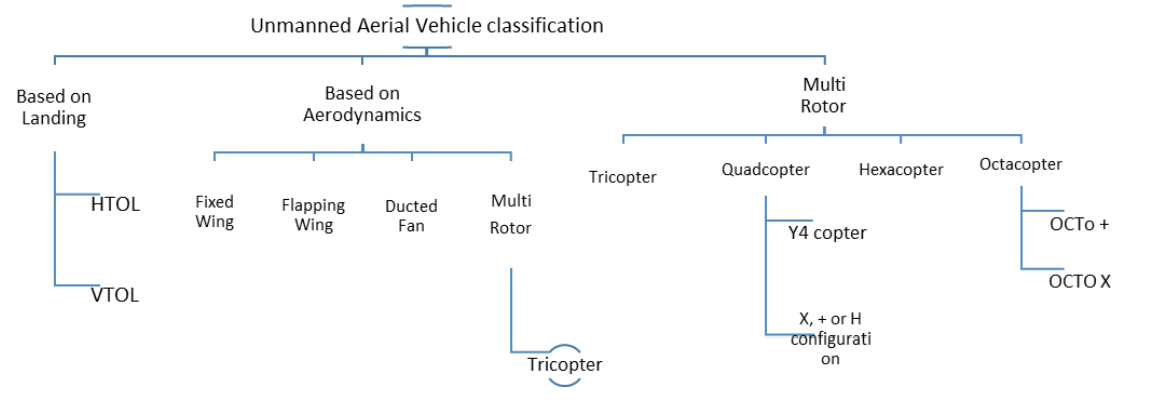
\includegraphics[width=0.7\textwidth]{Images/introducao/drone_classification.png}
  \caption{Classificação de VANTs por tipo de pouso, aerodinâmica e quantidade de rotores.}
  \label{fig:drone_classification.png}
\end{figure}

Como mostrado no organograma da figura acima~\ref{fig:drone_classification.png}, as categorias mais comuns para os VANTs são obtidas pelos atributos "tipo de pouso", "aerodinâmica" e "quantidade de rotores".

O tipo de aerodinâmica responsável pela sustentação das aeronaves no ar é bastante diversificado. Uma categoria bem comum de \textit{drones} são os VANTs de asa fixa, que semelhantemente aos aviões, tiram proveito da geometria das asas e da velocidade gerada por um ou mais motores para obterem sustentação. 

A classificaçao de aterrisagem, com a nomenclatura VTOL e HTOL diz respeito apenas aos VANTs de asa fixa visto que apenas esses tipos de VANTs tiram proveito tanto da aterrisagem vertical quanto da autonomia proveniente do vôo horizontal com asas fixas. 

No presente documento focaremos mais acetuadamente nos \textit{drones} de asa rotativa, visto que esse tipo de \textit{drone} será utilizado nos experimentos que sucederão.

\subsection{Componentes dos VANTs de Asa Rotativa}

Os componentes dos \textit{drones} de asa rotativa variam conforme o tipo de missão. Alguns dos componentes principais podem ser listados abaixo:

\begin{enumerate}
  \item Frame
  \item Motores e hélices
  \item Escs
  \item Controladora de voo
  \item Bateria e Placa distribuidora de energia
\end{enumerate}

\newpage

\subsubsection*{Frame}
\begin{figure}[H]
  \centering
  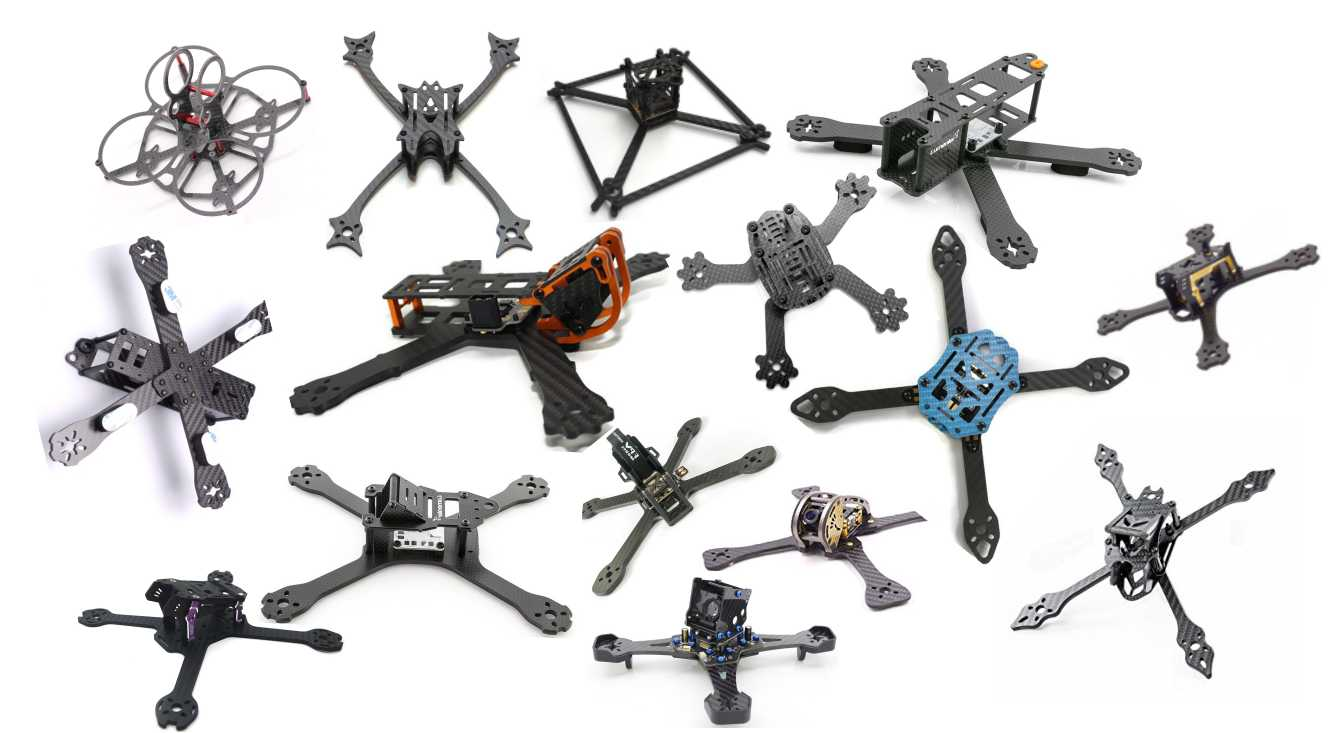
\includegraphics[width=0.7\textwidth]{Images/introducao/different_frames.jpg}
  \caption{Diferentes tipos de \textit{frames} (FONTE~\cite{url:esc_pwm}).}
  \label{fig:different_frames.jpg.0}
\end{figure}
%
O \textit{frame} de um \textit{drone} é a base estrutural na qual todos os outros componentes são fixados, ele pode possuir diversos formatos e tamanhos e geralmente é feito de um material leve e resistente como fibra de carbono ou polímeros plásticos. 

\subsubsection*{Motores e hélices}
%
\begin{figure}[H]
  \centering
  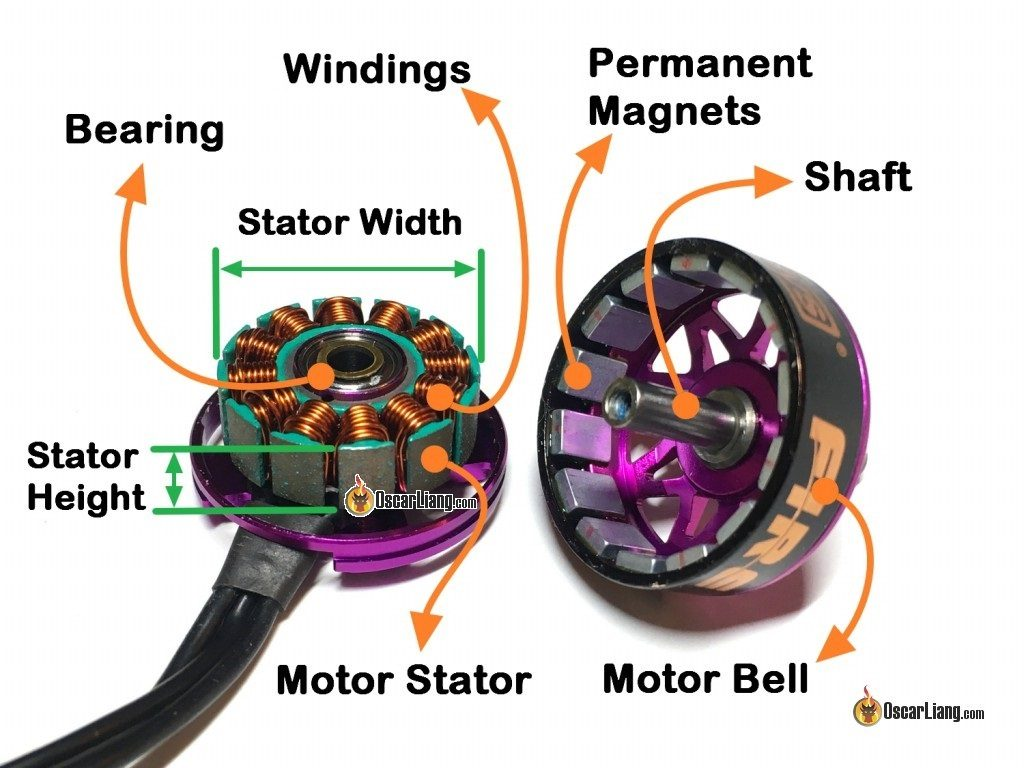
\includegraphics[width=0.5\textwidth]{Images/introducao/brushlessmotor.jpg}
  \caption{Motor DC Sem Escova (FONTE~\cite{url:brushless}).}
  \label{fig:brushlessmotor.jpg.0}
\end{figure}
%
Os motores do \textit{drone} são os responsáveis por converter a energia elétrica proveniente das baterias em energia cinética. Geralmente os 
motores utilizados são motores de corrente contínua não escovados (\textit{brushless DC}), por conta de seu tamanho reduzido e grande eficiência. O princípio de funcionamento desse tipo de motor reside na alternação da corrente em diferentes enrolamentos na parte interna dependendo da posição do eixo externo, esse processo é demonstrado na figura \ref{fig:brushlessscheme.jpg.0}. 
%
\begin{figure}[H]
  \centering
  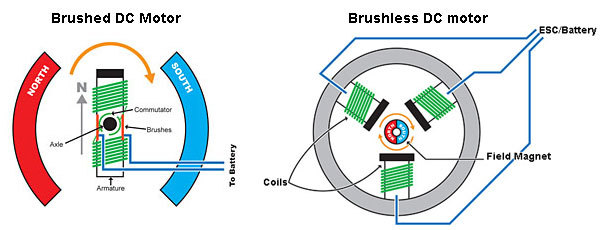
\includegraphics[width=0.6\textwidth]{Images/introducao/brushlessscheme.jpg}
  \caption{Princípio de Funcionamento do Motor DC Sem Escova (FONTE~\cite{url:brushlessscheme}).}
  \label{fig:brushlessscheme.jpg.0}
\end{figure}
%
A dinâmica de voo dos \textit{drones} de asa rotativa é bastante complexa, de forma resumida, a partir da corrente elétrica fornecida aos motores, eles movimentam as hélices, que devido à sua aerodinâmica geram uma força resultante para cima no \textit{drone}, a qual é denominada empuxo.  

%
\begin{figure}[H]
  \centering
  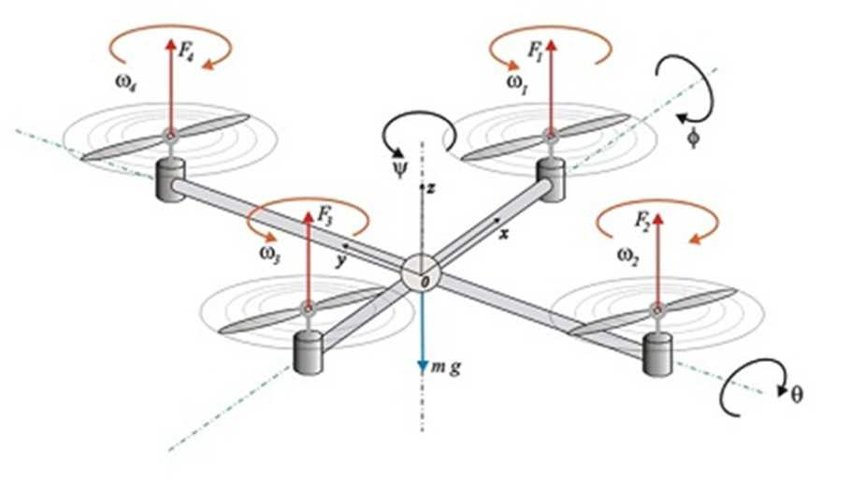
\includegraphics[width=0.6\textwidth]{Images/introducao/force_diagram_drone.png}
  \caption{Diagrama de Forças no Drone Quadricóptero (FONTE~\cite{url:drone_forces_diagram}).}
  \label{fig:force_diagram_drone.png.0}
\end{figure}
%
De forma mais detalhada, é possível descrever a dinâmica desse tipo de aeronave a partir do diagrama de forças e torques gerado por cada um dos motores como demonstrado na figura \ref{fig:force_diagram_drone.png.0}. Entretanto, a análise completa de tal dinâmica é extensa e não é o foco deste documento.  

\subsubsection*{ESCs}

Os ESCs (\textit{Eletronic Speed Controllers}) são os componentes eletrônicos responsáveis por controlar a velocidade dos motores. Eles são comandados pela controladora de voo, a partir de sinais PWM. Essa mesma modulação é utilizada pelo circuito do ESC para chavear o circuito entre bateria e motor. Esse chaveamento gera uma tensão resultante nos enrolamentos que controla o torque do motor. 
%
\begin{figure}[H]
  \centering
  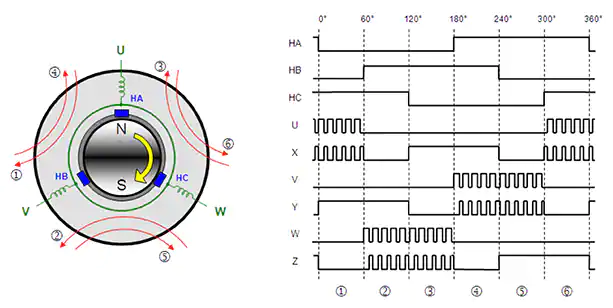
\includegraphics[width=0.6\textwidth]{Images/introducao/esc_wave_form.png}
  \caption{Formas de onda do ESC (FONTE~\cite{url:esc_wave_form}).}
  \label{fig:esc_wave_form.png.0}
\end{figure}
%
Como demonstrado na figura \ref{fig:esc_wave_form.png.0}, os motores \textit{brushless} são alimentados pela energização sequencial dos enrolamentos usando um sinal PWM. O ciclo de trabalho do sinal PWM é proporcional à tensão do drive. Na figura , “U”, “V” e “W” são os enrolamentos e “HA”, “HB” e “HC” são os sensores de efeito Hall de detecção de posição.
%
\begin{figure}[H]
  \centering
  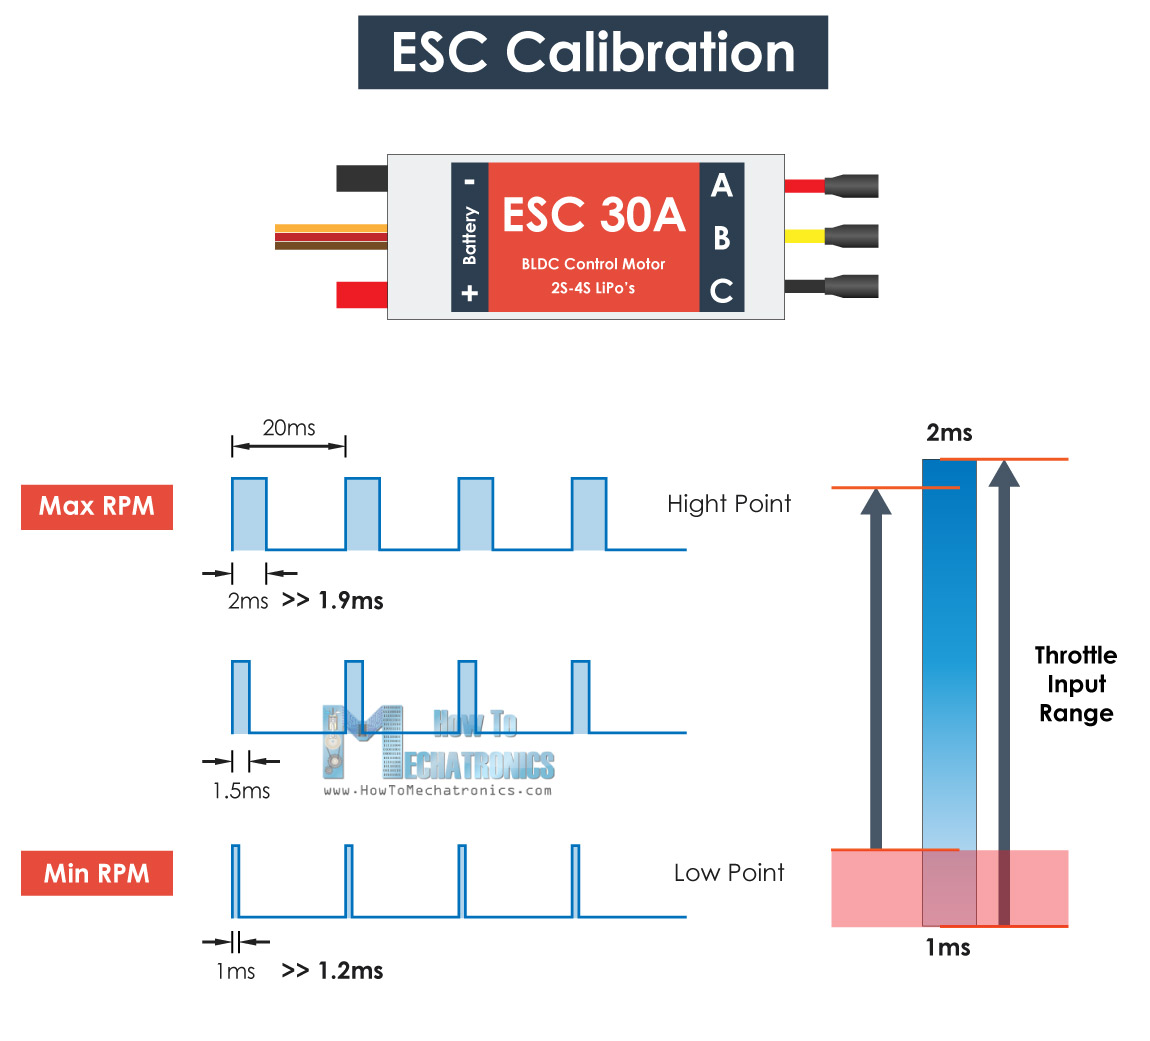
\includegraphics[width=0.6\textwidth]{Images/introducao/esc_pwm.jpg}
  \caption{PWM de Entrada do ESC (FONTE~\cite{url:esc_pwm}).}
  \label{fig:esc_pwm.jpg.0}
\end{figure}
%
O PWM produzido pela controladora de voo geralmente possui um intervalo de variação do ciclo de trabalho maior do que o necessário na entrada do ESC, a figura \ref{fig:esc_pwm.jpg.0} mostra a diferença dos intervalos de PWM mínimo e máximo produzidos pela controladora e o necessário para atingir a rotação mínima e máxima nos motores.

\subsubsection*{Controladora de Voo}

A controladora de voo é um microcontrolador com \textit{software} embarcado dedicado às funções básicas da aeronave. Ela possui sensores 
inerciais embutidos para comandar a dinâmica de voo da aeronave, além de possuir interface eletrônica com outros componentes como módulos \textit{GPS}, módulos receptores de rádio, módulos de telemetria entre outros. Sem a controladora de voo, seria uma tarefa humanamente impossível controlar o voo da aeronave, visto que a controladora depende de um \textit{feedback} contínuo e instantâneo dos parâmetros inerciais. 

\subsubsection*{Bateria e Placa distribuidora de energia}

A bateria é a fonte de energia do \textit{drone}, geralmente são utilizadas baterias Li-Po (Lítio-Polímero) pela sua boa relação massa/desempenho 
energético, essas baterias possuem uma nomenclatura específica com base na quantidade de células <explicar melhor as baterias>.

\subsection{\textit{ArduPilot}}
%
\begin{figure}[!htbp]
  \centering
  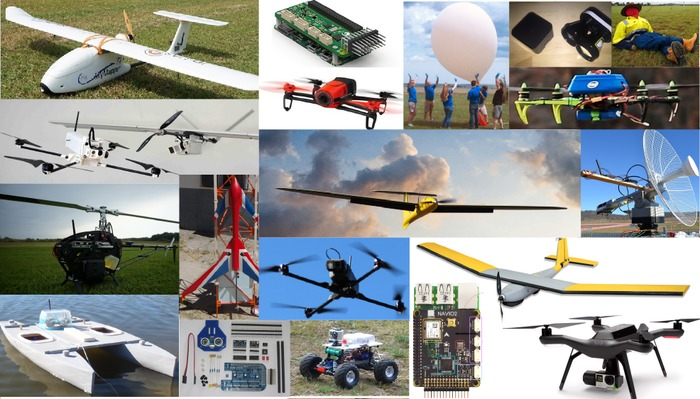
\includegraphics[width=0.7\textwidth]{Images/introducao/ardupilot_vehicles.jpg}
  \caption{Veículos suportados pelo \textit{ArduPilot}.}
  \label{fig:ardupilot_vehicles.jpg.0}
\end{figure}
%

O \textit{ArduPilot} é um projeto de código aberto que possui um conjunto de \textit{software} destinado ao piloto automático de veículos não tripulados, os quais incluem:
\begin{itemize}
  \item Plane - piloto automático para \textit{drones} de asa fixa.
  \item Copter - piloto automático para \textit{drones} de asa rotativa.
  \item Rover - piloto automático para veículos terrestres e barcos.
  \item Sub - piloto automático para veículos submarinos.
\end{itemize}

Além de suportar o \textit{firmware} para todos esses tipos de veículos, a comunidade \textit{ArduPilot} também se preocupa em desenvolver outras plataformas que auxiliam o desenvolvimento e a utilização do próprio \textit{firmware}, como por exemplo:

\begin{itemize}
  \item \textit{Antenna Tracker - firmware} para mirar uma antena automaticamente para o veículo.

  \item \textit{Mission Planner - interface} de estação de controle em solo escrita em C\# para Windows.
  
  \item \textit{APM Planner 2.0 - interface} de estação de controle específica para APM escrita em C++ usando os módulos Qt, pode ser executada em Linux, Windows e Mac.
  
  \item \textit{MAVProxy - interface} de estação de controle em linha de comando ou via \textit{script}.
  
  \item \textit{drone}Kit - APM SDK para aplicações executadas de forma embarcada, em mobile, e/ou na nuvem.
  
  \item \textit{MinimOSD} - visualização de informações de voo em tempo real no visor da interface de FPV.
  \item \textit{Tower} - interface de estação de controle para celular.  
  \item \textit{QGroundControl} é uma interface de estação de controle alternativa escrita em C++ usando os modulos Qt.
  \item \textit{PX4 - firmware pixhawk} para a controladora \textit{pixhawk}.
  
  \item \textit{MAVlink} - o protocolo para comunicação entre estação de controle, controladora de voo e alguns componentes incluindo OSD.
  
  \item \textit{UAVCAN} - protocolo leve e confiável para aplicações de comunicação aeroespacial e robótica, via \textit{CAN bus}. 
  
\end{itemize}

A lista de placas eletrônicas compatíveis com o \textit{firmware} \textit{ArduPilot} pode ser encontrada na documentação, no seguinte endereço ~\cite{url:ardupilotdoc}. 


\subsection{UART}

UART, que vem das palavras \textit{universal asynchronous receive/transmit}, realiza o papel principal na comunicação serial, já que converte os dados entre série e paralelo. Há então uma conversão de paralelo-serial para os dados transmitidos, e uma outra serial-paralelo para os dados recebidos. Existe ainda um \textit{buffer}, cujo objetivo é armazenar dados por tempo limitado em transmissões com alta taxa, sem que haja descarte de dados e consequente perda de informação. Para que não haja fluxo de transmissão caso ambas as partes não estiverem prontas, em adição as características citadas, são incorporados circuitos reguladores de fluxo.

A divisão do protocolo é feita em três sub-módulos, gerador de taxa de transmissão, módulo de transmissão e módulo de recepção. O primeiro, se responsabiliza por gerar um sinal de relógio localmente, o qual deve ser muito maior que a taxa de transmissão de dados entre transmissor-receptor. O módulo receptor, por sua vez, recebe os sinais RXD e os converte para dados paralelos. Por fim, o módulo transmissor converte os bytes em \textit{bits} seriais, com base no padrão de quadro utilizado, e os envia através de sinais TXD. \cite{uart}

\subsection{Telemetria}

A telemetria é uma funcionalidade indispensável nos \textit{drones} mais modernos, ela permite receber informações dos sensores do \textit{drone} em tempo real como altitude, velocidade, gps, temperatura, informações da quantidade de carga na bateria dentre outras. No  \textit{hardware} do \textit{drone}, essa transmissão de dados geralmente é feita por um módulo dedicado a isso ou então em módulos receptores de rádio que já possuem essa funcionalidade integrada. Uma controladora com \textit{firmware ArduPilot} utiliza o protocolo \textit{MAVlink} para o envio das mensagens de telemetria.

\subsection{Protocolo \textit{MAVlink}}

\textit{MAVlink} é um protocolo de comunicação com \textit{drones} e entre os componentes acoplados ao \textit{drone}. Essa transmissão consiste no envio de um fluxo de dados, os quais são chamados de tópicos, e escritos em arquivos XML. Dentre as principais vantagens de se utilizar o \textit{MAVlink} estão a sua eficiência e versatilidade. Em números, a segunda versão do \textit{MAVlink} tem apenas 14 \textit{bytes} de \textit{overhead} no pacote de comunicação. Além disso, provê métodos de detectar perda de pacotes e dados corrompidos, e garante a autenticação dos pacotes. Outro ponto positivo é o suporte a diversas linguagens, já que o protocolo tem suporte a diferentes tipos de sistemas operacionais e microcontroladores. Por fim, apesar de menos importante para o nosso projeto, vale citar que o protocolo suporta até 255 usuários simultâneos em uma mesma rede.
\cite{MAVlink}

\subsection{Computadores de Bordo}

Computadores de bordo (ou \textit{Companion Computers}, como são chamados na documentação do \textit{ArduPilot}) podem ser utilizados para interfacear com o \textit{firmware ArduPilot} numa controladora de voo através do protocolo \textit{MAVlink}. Dessa forma, o computador de bordo consegue computar todos os dados \textit{MAVlink} produzidos pela controladora e com estes pode fazer decisões inteligentes durante o voo. 

Geralmente, no quesito de hardware para esses computadores são escolhidos mini computadores de arquitetura baseada em ARM. Os mini computadores suportados pela comunidade \textit{ArduPilot} são listados abaixo:

\begin{itemize}
  \item \textit{Arduino family}
  \item \textit{LYCHEE (Cube Carrier Board for Raspberry Pi Compute Module)}
  \item NVidia TX1
  \item NVidia TX2
  \item \textit{ODroid}
  \item \textit{Raspberry Pi}
\end{itemize}

Já no quesito de \textit{software}, existem ferramentas, programas e sistemas operacionais específicos para computadores de bordo, tais programas conseguem computar os dados \textit{MAVlink} vindos da controladora. Alguns dos softwares suportados pela comunidade \textit{ArduPilot} são listados abaixo:

\begin{itemize}
  \item APSync
  \item \textit{drone}Kit
  \item FlytOS
  \item Maverick
  \item ROS
  \item Rpanion-server
\end{itemize}


\subsection {Série de computadores \textit{Raspberry Pi}}
%
O \textit{Raspberry Pi} é uma série de computadores de placa única e tamanho reduzido, que recebem a denominação  SoC (\textit{System on Chip})~\cite{url:soc} à qual são conectados os seguintes dispositivos: monitor, teclado, e mouse. 

Desenvolvido no Reino Unido pela \href{https://www.raspberrypi.org/}{Raspberry Pi Foundation} tendo, como principais objetivos, contribuir para inclusão digital, promoção de ensino básico em ciência da computação e empoderamento social. Uma alternativa de ensino com baixo custo para escolas e estudantes~\cite{url:raspberry_wiki}. A Tabela~\ref{tab:Especificacoes} apresenta as especificações técnicas do modelo \textit{Raspberry Pi Revision 2 - Element 14}.
%
\begin{table}[!htbp]
    \centering
    \begin{tabular}{ |c|c| } 
        \hline
        Chip & Broadcom BCM2835 SoC Full HD Processador de Aplicações Multimídia\\
        \hline
        CPU & 700 Mhz ARM1176JZ-F Processador de Baixa Potência de aplicações \\
        \hline
        GPU & Dois Núcleos, VideoCore IV, Co-Processador de Multimídia \\ 
        \hline
        Memória & 512MB SDRAM  \\
        \hline
        Ethernet & Onboard 10/100 Ethernet com conector RJ-45 \\
        \hline
        USB 2.0 & Dois Conectores USB 2.0 \\ 
        \hline
        Saída de Vídeo & HDMI e Composição RCA (PAL e NTSC) \\ 
        \hline
        Saída de Áudio & Conector 3.5 mm ou HDMI \\
        \hline
        Armazenamento & SD, MMC, SDIO Card Slot \\
        \hline
        Dimensões & 8.6 cm X 5.4 cm X 1.7 cm \\ 
        \hline
    \end{tabular}
    \caption{Especificações técnicas do modelo \textit{Raspberry Pi Revision 2 - Element14}.}
    \label{tab:Especificacoes}
\end{table}

\pagebreak

Na Figura~\ref{fig:rasp3b.jpg.0} é mostrado uma fotografia do modelo. 
Dentre os 25 Pinos presentes neste Raspberry, 17 podem ser usados como entradas ou saídas de uso geral, 5 como terminais comuns (GND), 2 como fontes de tensão de valor +5V e 2 como fontes de tensão de valor +3.3V. 

%
A Tabela~\ref{tab:Raspberry Pinout} reúne uma descrição de todos os pinos.
%
\begin{figure}[!htbp]
    \centering
    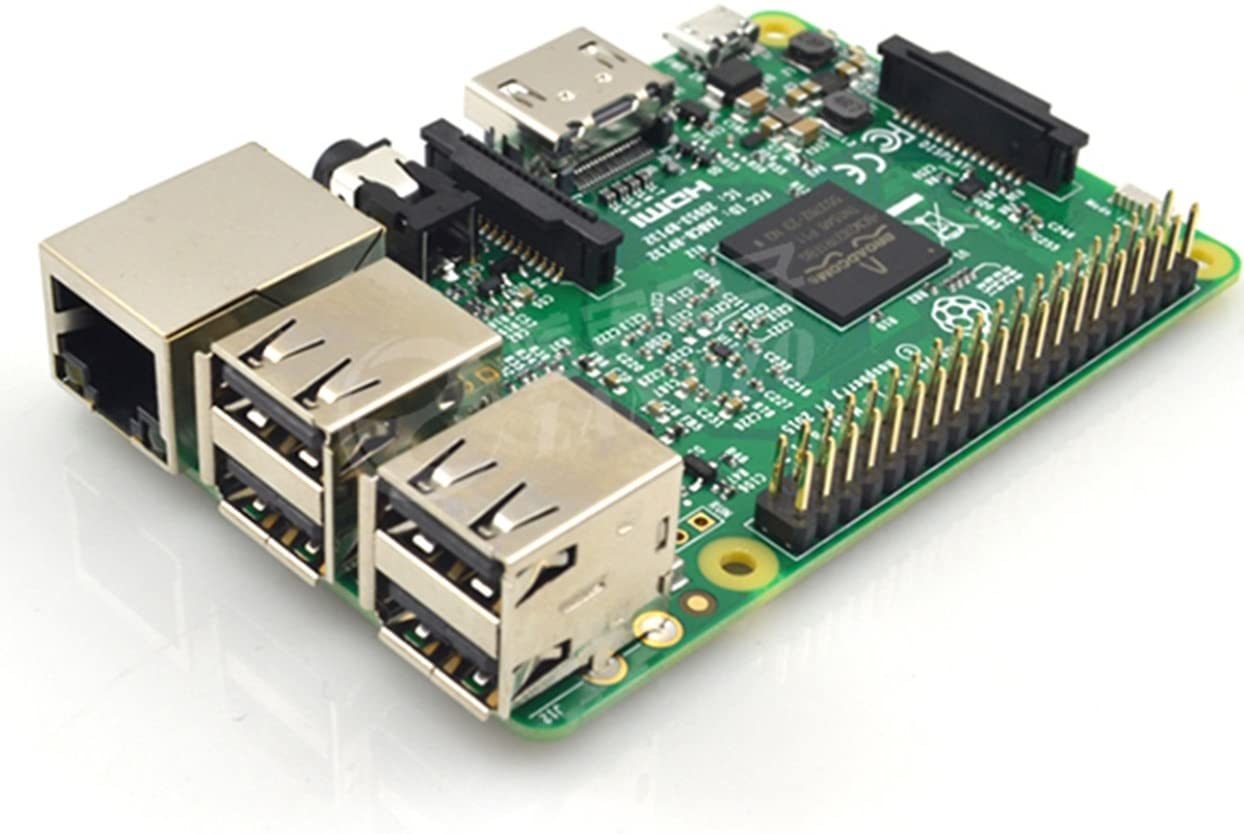
\includegraphics[width=0.7\textwidth]{Images/introducao/rasp3b.jpg}
    \caption{\textit{Raspberry Pi Revision 2.0}.}
    \label{fig:rasp3b.jpg.0}
\end{figure}
%
\begin{table}[!htbp]
    \centering
    \begin{tabular}{|c|c|c|c|} 
         \hline
         \textbf{N} & \textbf{Descrição} & \textbf{N} & \textbf{Descrição} \\ [0.5ex]
         \hline
         1 & Saída de +3.3V & 14 & Terminal Comum GND\\
         \hline
         2 & Saída de +5V & 15 & GPIO22 \\
         \hline
         3 & GPIO2 | Pull-Up | I2C-SDA & 16 & GPIO23 \\ 
         \hline
         4 & Saída de +5V & 17 & 3V3 \\
         \hline
         5 & GPIO3 | Pull-Up | I2C-SCE & 18 & GPIO24 \\
         \hline
         6 & Terminal Comum GND & 19 & GPIO10 | SPI | MOSI \\ 
         \hline
         7 & GPIO4 & 20 & Terminal Comum GND \\ 
         \hline
         8 & GPIO14 | UART | TXD & 21 & GPIO9 | SPI | MISO\\
         \hline
         9 & Terminal Comum GND & 22 & GPIO25\\
         \hline
         10 & GPIO15 | UART | RXD & 23 & GPIO11 | SPI | CLK\\ 
         \hline
         11 & GPIO17 | UART-RTS & 24 & GPIO8 | SPI | CE0\\
         \hline
         12 & GPIO18 | PWM & 25 & Terminal Comum GND\\ 
         \hline
         13 & GPIO27 & 26 & GPIO7 | SPI | CE1\\ 
         \hline
    \end{tabular}
    \caption{Descrição dos pinos do \textit{Raspberry Pi Rev 2.0 - Element 14}.}
    \label{tab:Raspberry Pinout}
\end{table}


\subsection{ROS - Robot Operative System}

Robot Operating System, ROS ou ros, é um \textit{middleware}, 
com foco em robótica, \textit{open-source}. O ROS não é considerado 
um sistema operacional, mas um conjunto de \textit{software 
frameworks} para desenvolvimentos de \textit{softwares} para robôs. 
Oferece serviços a uma vasta gama de computadores, 
como abstração de hardware, controle de dispositivos 
de baixo nível, implementação de funcionalidades usadas 
comumente, troca de mensagens entre processos e 
gerenciamento de pacotes. A arquitetura de grafos 
pode ser usada para representar processos baseados 
em ROS, onde os processos são tidos como vértices, 
os quais podem receber, enviar, e multiplexar 
dados de sensores, controlar, planejar e trocar 
outras mensagens. Apesar da necessidade de baixa latência
e interações rápidas, o ROS não é um \textit{Real-Time
Operating System} (RTOS). Entretanto, embora pouco explorado,
é possível integrar códigos executados em tempo real.
Essa falta de um suporte nativo a códigos de tempo real é
uma preocupação real dos desenvolvedores, os quais planejam 
integrá-los ao ROS 2, projeto que visa ter proveito de 
bibliotecas e tecnologias mais novas. 

As principais bibliotecas do ROS são voltadas para sistemas
Unix, isso se deve ao fato da dependência com diversos
\textit{softwares open-source}. Para essas bibliotecas,
o Ubuntu é listado como "\textit{supported}", entretanto,
para outras distros Linux, como o Fedora, macOS e Windows,
todos são listados como "\textit{experimental}". Ainda assim,
existem exceções, como a biblioteca rosjava, a qual foi 
escrita para Android OS. Apesar disso, oferece uma integração
nativa com o MATLAB, programa que pode ser usado no Linux,
macOS ou Windows. Outro caso a parte é a biblioteca roslibjs,
voltada para desenvolvimento \textit{web} com JavaScript,
que garante compatibilidade com qualquer navegador padrão.


\subsection{\textit{MAVROS}}

\textit{MAVROS} é um pacote do ROS cujo objetivo é habilitar a comunicação de computadores que rodam ROS e qualquer outro dispositivos que se comunique usando o protocolo \textit{MAVlink}. Em outras palavras, o \textit{MAVROS} converte tópicos do ROS em mensagens \textit{MAVlink}, permitindo que, por exemplo, VANTs que usam o ArduPilot se comuniquem com o ROS.  \cite{mavros}

<listar os tópicos>

\subsection{Django}

Django é um \textit{web framework} cuja intenção é tornar o desenvolvimento \textit{web} mais veloz e fácil. Possui uma integração nativa entre banco de dados, \textit{front-end} e \textit{back-end}, apesar de que não seja necessária a utilização de um banco de dados. Primeiramente, podemos citar que todo o esquema do banco é feito através de códigos \textit{python}, pela técnica de mapeamento objeto-relacional, como podemos ver no exemplo a seguir\cite{django}.

\begin{lstlisting}[language=Python]
from django.db import models

class Reporter(models.Model):
    full_name = models.CharField(max_length=70)

    def __str__(self):
        return self.full_name

class Article(models.Model):
    pub_date = models.DateField()
    headline = models.CharField(max_length=200)
    content = models.TextField()
    reporter = models.ForeignKey(Reporter, on_delete=models.CASCADE)

    def __str__(self):
        return self.headline
\end{lstlisting}

No exemplo acima, são instanciadas duas tabelas, \textit{Reporter} e \textit{Article}, e suas respectivas colunas. A fim de criá-las no banco deve-se executar os comandos:

\begin{lstlisting}[language=bash] 
$ python manage.py makemigrations
$ python manage.py migrate
\end{lstlisting}

A partir do momento que os modelos estão criados, podemos registrá-los no arquivo referente ao administrador, o que possibilita a criação, alteração e remoção dos objetos através da \textit{interface web} criada pelo próprio Django. Para habilitar as operações citadas sobre a classe \textit{Article}, por exemplo, basta configurar o arquivo \textit{admin.py} tal como:

\begin{lstlisting}[language=Python]
from django.contrib import admin

from . import models

admin.site.register(models.Article)
\end{lstlisting}

Outro ponto interessante é a possibilidade de configuração de \textit{URLs}. Para isso, devemos criar um código de mapeamento de \textit{URLs} dentro do arquivo \textit{urls.py}, como exemplificado a seguir:

\begin{lstlisting}[language=Python]
from django.urls import path

from . import views

urlpatterns = [
    path('articles/<int:year>/', views.year_archive),
    path('articles/<int:year>/<int:month>/', views.month_archive),
]
\end{lstlisting}

\newpage

\section{Arquitetura do sistema proposto}

%
\begin{figure}[!htbp]
  \centering
  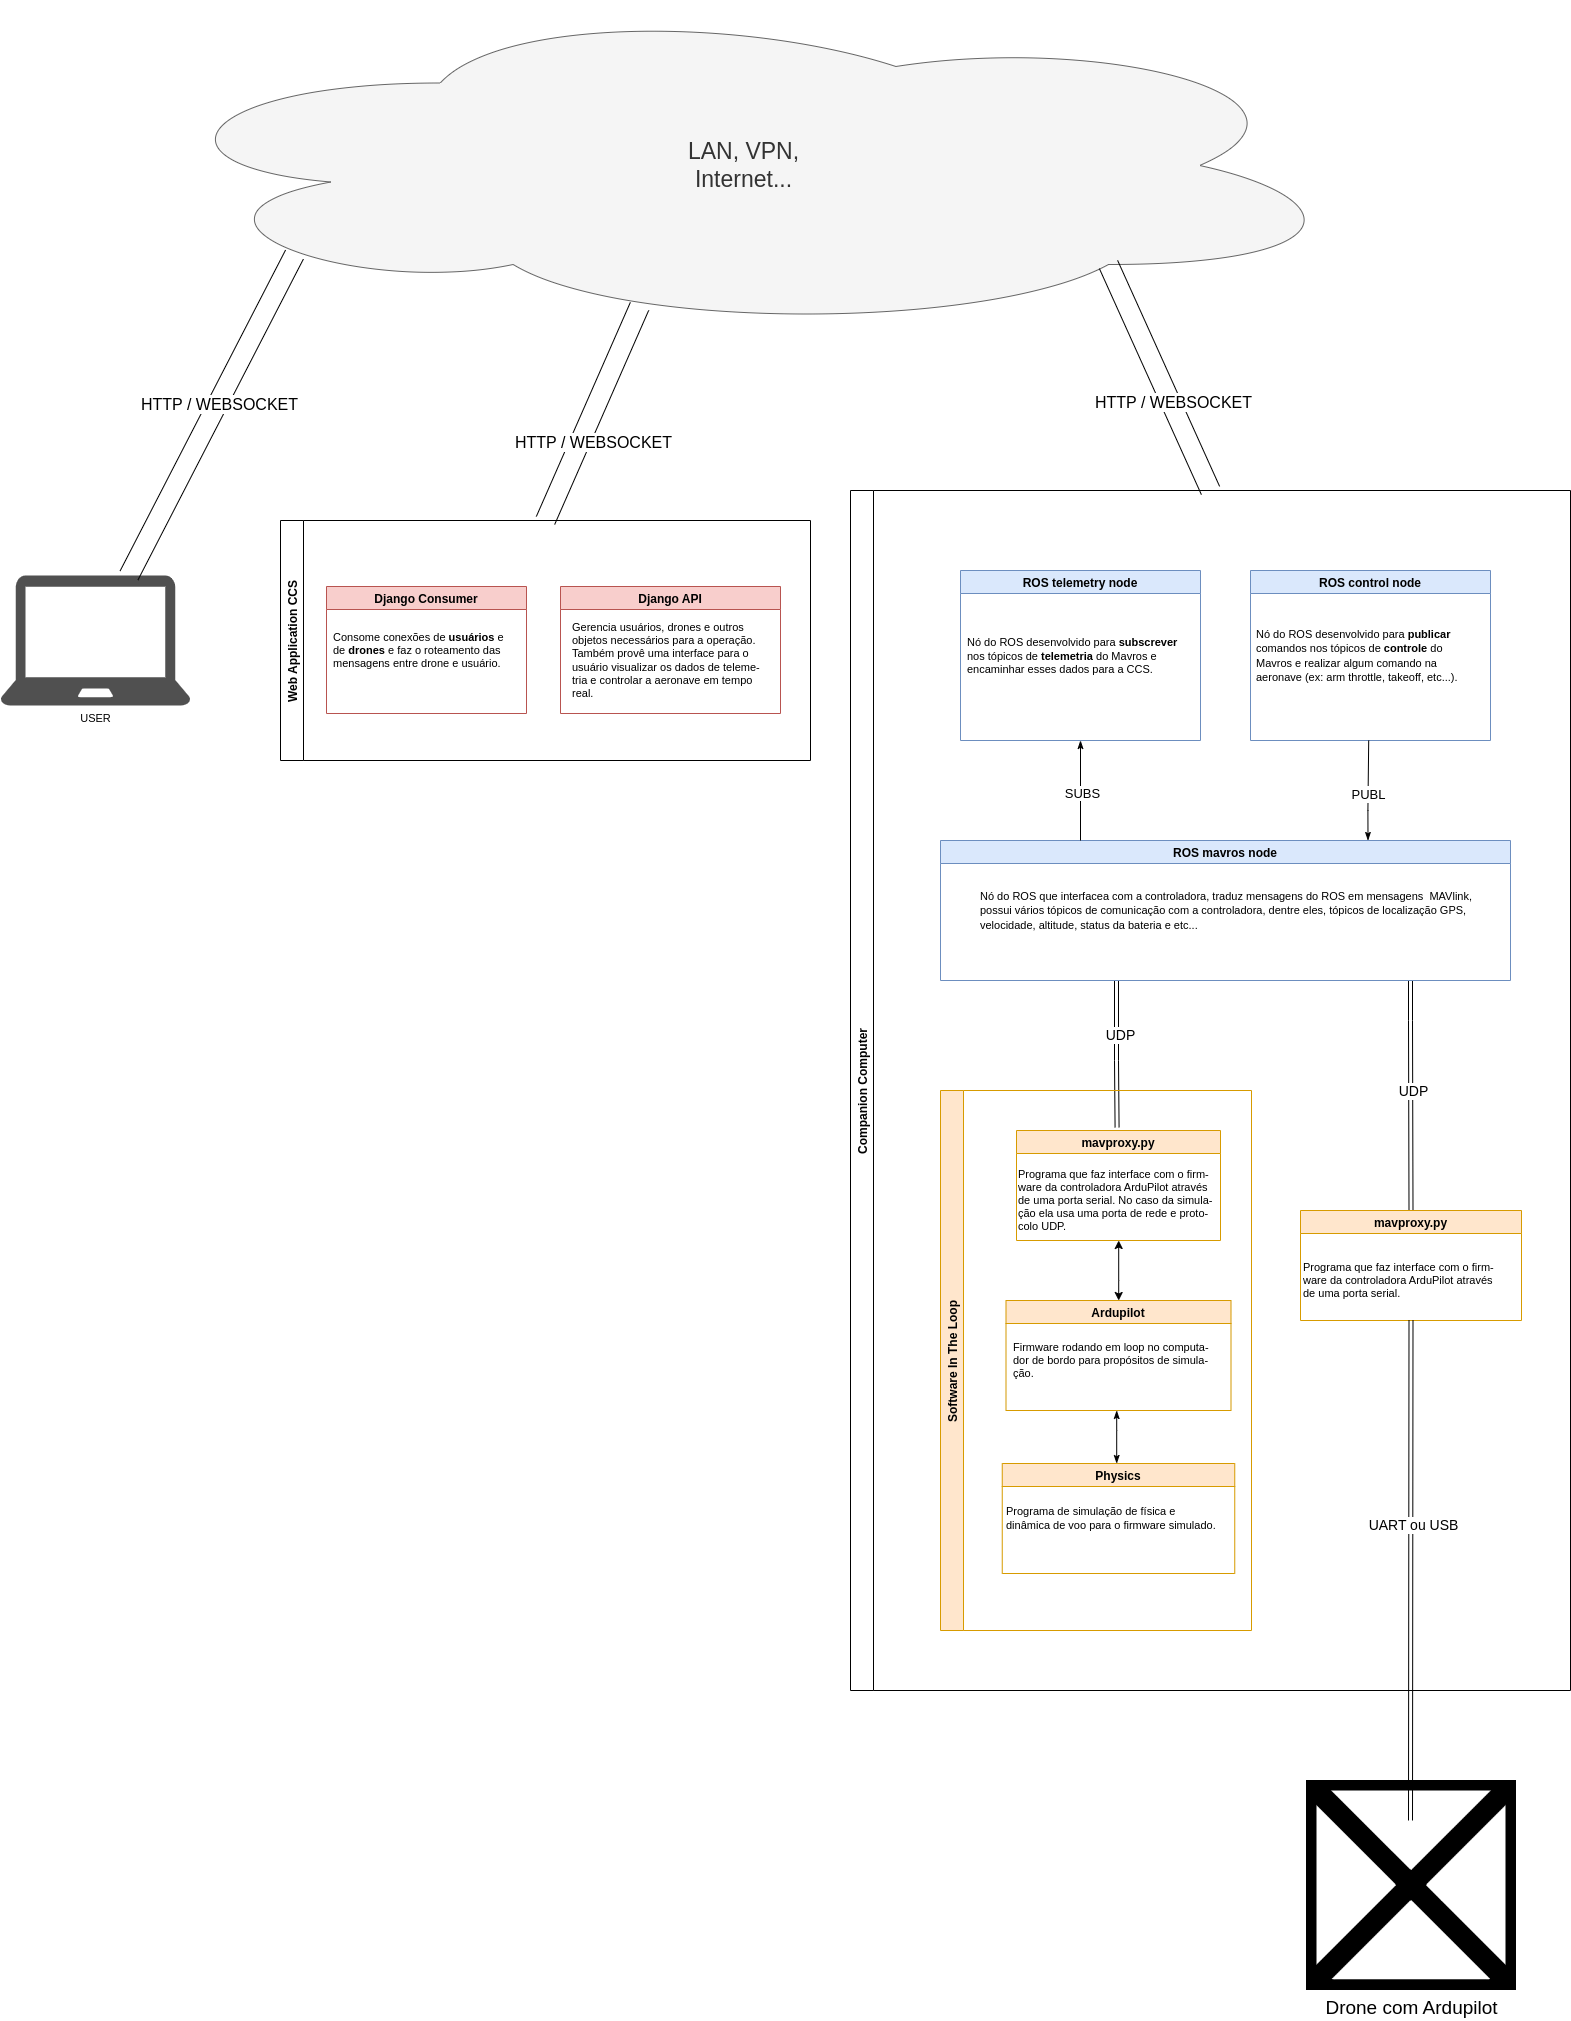
\includegraphics[width=1\textwidth]{Images/Diagramas/CCS_ARQ.png}
  \caption{Arquitetura da Aplicação.}
  \label{fig:CCS_ARQ.png.0}
\end{figure}
%


A partir do processo de pesquisa e também considerando os requerimentos da aplicação, o diagrama de arquitetura foi idealizado como demonstrado na figura \ref{fig:CCS_ARQ.png.0}. A API de controle e navegação foi batizada com o nome \textit{CCS}, que significa em inglês \textit{Cloud Control Station}, que vem da sigla já conhecida na comunidade \textit{ArduPilot} como \textit{GCS} de \textit{Ground Control Station}.   

O modelo cliente-servidor foi o escolhido para a aplicação pois, visto a natureza diversa da rede a qual o usuário e o \textit{drone} (os clientes) podem estar conectados, esse modelo pode ser aplicado em uma maior variedade de casos. Por exemplo, esse tipo de arquitetura de aplicação exige apenas que o servidor seja acessível na rede, e que tanto o \textit{drone} quanto o usuário consigam conectar-se a ele, enquanto que o modelo par-a-par ou híbrido exige que todas as partes sejam acessíveis e consigam comunicar-se umas com as outras, o que é mais difícil devido à configurações de \textit{firewall} e \textit{NAT} às quais os clientes podem estar submetidos. Dessa forma, este modelo se mostrou o ideal para desenvolver a aplicação, que por sua vez poderá ser acessada através de diversas formas como por meio de LAN, VPN, \textit{Internet} inclusive por dispositivos móveis utilizando a rede celular.

Partindo do modelo cliente-servidor, decidiu-se utilizar dois tipos de protocolos de aplicação para realizar a comunicação entre usuários, drones e API. O HTTP é utilizado para realizar chamadas à \textit{rest} API, que por sua vez autentica o usuário ou \textit{drone} que a chama e responde com o método \textit{rest} solicitado. Além desse protocolo, também utiliza-se o \textit{websocket} para realizar a comunicação entre usuário e \textit{drone} por intermédio da API. Nesse sentido, o HTTP é mais utilizado para funções de interface e funções administrativas do usuário para a API, enquanto o \textit{websocket} foi o escolhido para lidar com fluxo de dados de telemetria e comandos entre usuário e \textit{drone}. 

Para conectar \textit{drone} à API, no computador de bordo, serão desenvolvidos dois nós de ROS que farão interface com o \textit{MAVros}. O primeiro nó responsável apenas por transmitir dados de telemetria para a API e o segundo responsável por receber os comandos da API e comandar a controladora de voo. Escolheu-se separar as funções em dois processos distintos para garantir a independência entre as duas atividades e manter a resiliência da aplicação. Por fim, o nó \textit{MAVros} fará a comunicação com a controladora de voo através do \textit{MAVProxy}.



%    \centering
%    \includegraphics{Images/introducao/planta_inicial.png}
%    \caption{Diagrama em blocos da planta didática em configuração original.}
%    \label{fig:planta_inicial}
%\end{figure}


%%%%%%%%%%%%%%%%%%%%%%%%%%%%%%%%
%%%%%%%% Metodologia %%%%%%%%%%%
%%%%%%%%%%%%%%%%%%%%%%%%%%%%%%%%

\chapter{Metodologia}
\label{chapter:Metodologia e análise de trabalho semelhantes}
%
% retira numeracao da pagina, conforme as normas de apresentacao.
\thispagestyle{empty} 
%
\section{Pesquisa}
%
A pesquisa para elaboração deste projeto é em sua maior parte baseada nas documentações disponibilizadas pelas comunidades do \textit{ArduPilot}, \textit{ROS} e \textit{Django}. Existem vários exemplos da integração entre \textit{Django} e \textit{ROS} utilizando o protocolo \textit{websocket}, o exemplo tomado como base para a aplicação desenvolvida nesse documento pode ser acessado no seguinte endereço: \cite{url:django_ros}.
%
%\section{Objetivos do método aplicado}
A partir do processo de pesquisa e desenvolvimento, espera-se chegar a uma primeira versão funcional da aplicação de controle e navegação para \textit{drones} proposta no diagrama da figura \ref{fig:CCS_ARQ.png.0}.

\section{Abordagem}
Adotar-se-á uma análise qualitativa dos resultados obtidos a partir da implementação do novo sistema, em observância aos seguintes questionamentos:
\begin{enumerate}
    \item Com o sistema desenvolvido será possível receber dados de telemetria via rede?
    \item Com o sistema desenvolvido será possível ao operador do sistema, controlar o \textit{drone} remotamente?
    \item O quão seguro é o sistema desenvolvido? Quais riscos de segurança estão submetidos a tal sistema?
    \item pergunta avaliativa 3 TODO#
    \item pergunta avaliativa 4 TODO#
\end{enumerate}
%
%%%%%%%%%%%%%%%%
%

\section{Descrição do problema}
De forma resumida, deseja-se, a partir de um \textit{drone} montado com todos os seus componentes essenciais, acoplar um \textit{Raspberry Pi} à controladora do \textit{drone} para conectar o conjunto à rede de computadores e com isso expandir suas capacidades. Algumas questões surgem quanto a esse projeto, como por exemplo: Qual arquitetura de \textit{software} a ser utilizada, ou seja como o \textit{software} a ser desenvolvido será organizado? Qual arquitetura de rede a ser utilizada, por exemplo, par-a-par ou cliente-servidor? No quesito de comunicação na \textit{Internet}, na qual muitas vezes não se tem o controle da rede, como seria feita essa comunicação?

\section{Trabalhos correlacionados}

\textit{Cellular Controlled Drone Experiment: Evaluation of Network Requirements}\cite{artigo_relacionado_1} é um exemplo de documento acadêmico que se assemelha ao nosso trabalho. Na tese de mestrado, é investigada a possibilidade de conectar um \textit{drone} a uma rede IP, via \textit{Internet} móvel, mais especificamente pela tecnologia LTE (4G). Dentre os assuntos discorridos estão a construção, teste, análise dos resultados e, por fim, comparação com o modelo tradicional de comunicação, via controle remoto. 

O destaque do documento é a prova de conceito constatada pelos resultados obtidos. O \textit{drone} não só conseguiu ser controlado com uma latência aceitável, mas inclusive transmitir vídeo em tempo real a uma taxa de bits alta o suficiente para atingir uma qualidade razoável. Outro ponto importante mencionado no documento para evitar perdas ou atrasos de pacotes por conta de uma possível rede congestionada, é a criação de uma nova classe QCI para comunicações com \textit{drone}. \textit{QoS Class Identifier}, QCI, define o quão priorizado será o tráfego o canal, portanto, em redes com grande quantidade de usuários, é indispensável priorizar a comunicação com os \textit{drones}. 

Por fim, o artigo foi escrito em 2015 e muitas tecnologias surgiram desde então, tal como o 5G. Assim sendo, a mesma metodologia de pesquisa e testes podem ser feitas utilizando a rede 5G a fim de comparar os resultados e constatar se houve um ganho significativo entre gerações.



%%%%%%%%%%%%%%%%%%%%%%%%%%%%%%%%%%%%%%%%%%%%%%%%%%%%%%%
%
\chapter{Detalhamento da solução}
%
% retira numeracao da pagina, conforme as normas de apresentacao.
\thispagestyle{empty} 
%

\section{Ambiente de simulação}
%
\begin{figure}[!htbp]
  \centering
  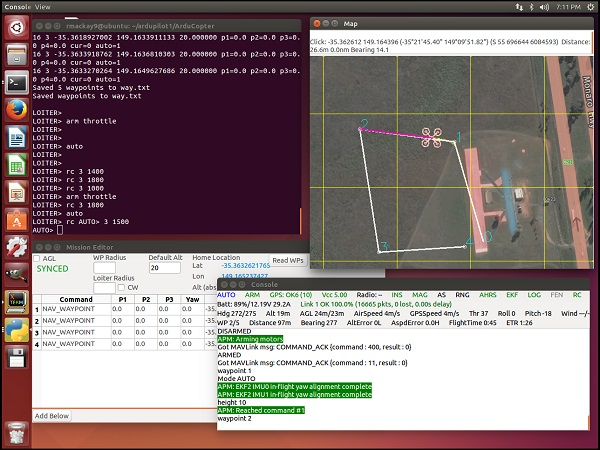
\includegraphics[width=0.7\textwidth]{Images/Desenvolvimento/sitl_demo.jpg}
  \caption{Demonstração do \textit{Software In The Loop}.}
  \label{fig:sitl_demo.jpg.0}
\end{figure}
%

O projeto \textit{ArduPilot} possui um rico conjunto de ferramentas que auxiliam no desenvolvimento de aplicações para \textit{drones}. O próprio código fonte do \textit{firmware} \textit{ArduPilot} pode ser compilado e carregado em um ambiente de simulação. O executável responsável por isso é chamado SITL (\textit{Software In The Loop}), cujo digrama é apresentado na figura \ref{fig:sitl_arq.jpg.0}, esse programa consegue integrar-se com outros formando um ambiente de simulação completo. O \textit{MAVProxy} é utilizado para fazer a interface de comunicação entre o operador e a controladora em ambiente simulado. Além disso, é possível integrar com um simulador de física e dessa forma simular a dinâmica de voo da aeronave. A simulação da dinâmica de voo da aeronave geralmente vem acompanhada com a integração de algum \textit{software} de visualização como no caso do Flight Gear e do Gazebo, o qual estaremos utilizando. A integração de todos esses componentes no ambiente de simulação forma um loop, e com isso temos o nome \textit{Software In The Loop}. Essa aplicação é essencial para o desenvolvimento pois permite a execução do \textit{ArduPilot} sem a utilização de nenhum hardware.

%
\begin{figure}[H]
  \centering
  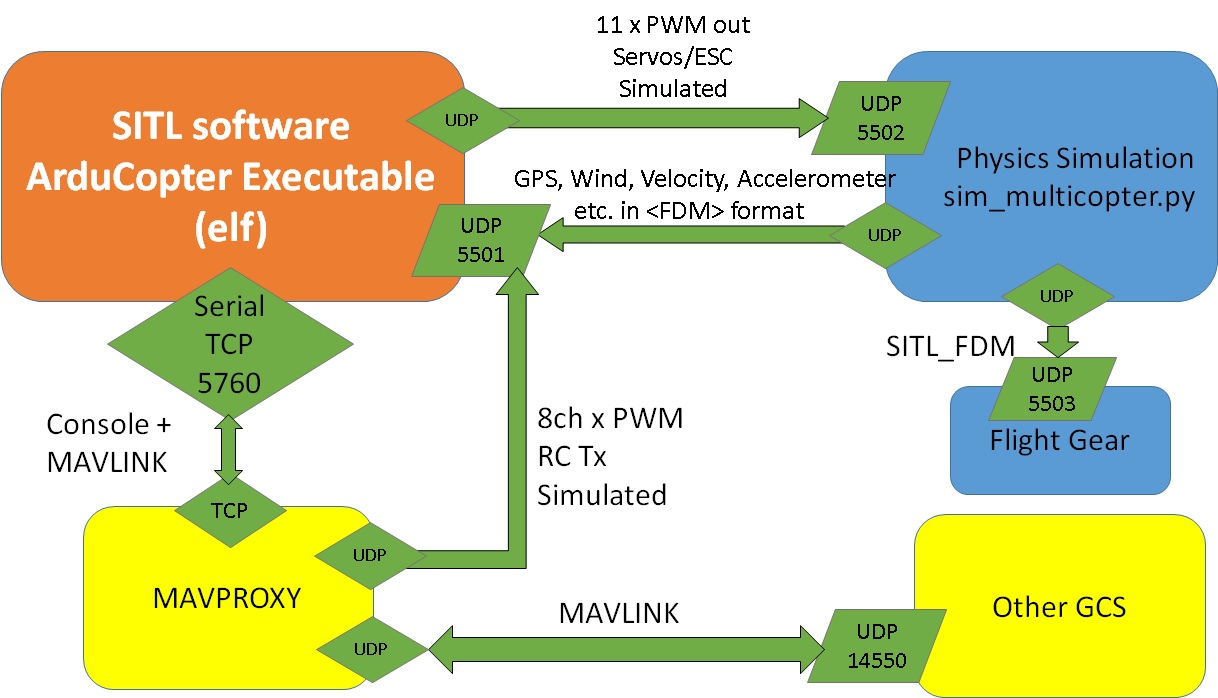
\includegraphics[width=0.7\textwidth]{Images/Diagramas/sitl_arq.jpg}
  \caption{Arquitetura do \textit{Software In The Loop}}
  \label{fig:sitl_arq.jpg.0}
\end{figure}
%



A inicialização do SITL é feita utilizando o script python demonstrado na figura \ref{fig:sim_vehicle.png.0}, que é disponibilizado junto ao código fonte do \textit{ArduPilot} no seu repositorio do github.

%
\begin{figure}[H]
  \centering
  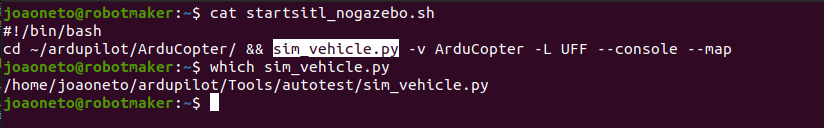
\includegraphics[width=0.7\textwidth]{Images/Desenvolvimento/sim_vehicle.png}
  \caption{sim\_vehicle.py}
  \label{fig:sim_vehicle.png.0}
\end{figure}
%

Como demonstrado na figura \ref{fig:sim_vehicle.png.0} criamos um script bash para executar o ambiente de simulação, nos parâmetros especificamos que queremos simular o firmware ArduCopter, utilizando as interfaces de mapa e console. Além disso, inserimos como parametro a localização em coordenadas do campo de futebol da UFF no Campus de Gragoatá. O resultado da execução desse script pode ser visualizado na figura \ref{fig:startsitl_nogazebo.png.0}.

%
\begin{figure}[H]
  \centering
  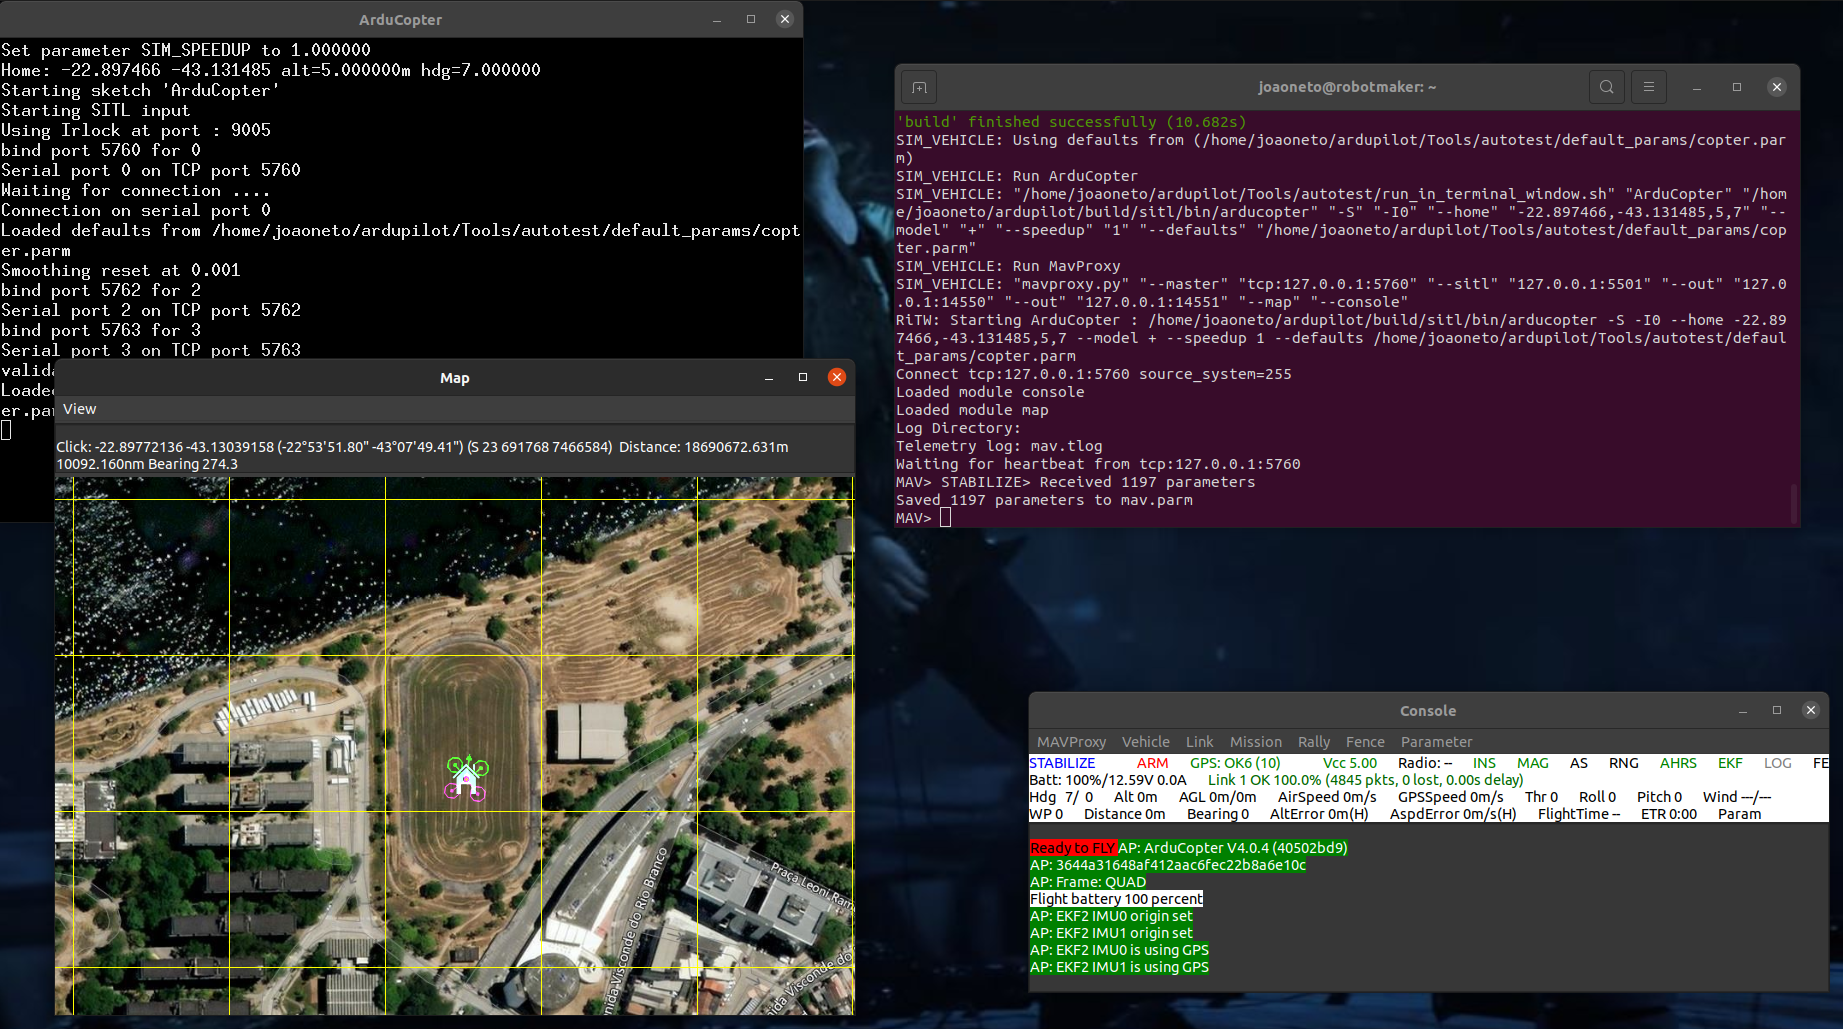
\includegraphics[width=0.8\textwidth]{Images/Desenvolvimento/startsitl_nogazebo.png}
  \caption{startsitl\_nogazebo.sh}
  \label{fig:startsitl_nogazebo.png.0}
\end{figure}
%

Fizemos também um segundo script bash com os parâmetros necessários para a conexão com o Gazebo, que é o \textit{software} que simula um mundo em 3D para o \textit{drone}. Separamos nesses dois scripts, pois na maioria das vezes a simulação em 3D nao é necessária e consome muito dos recursos da máquina que a executa.

%
\begin{figure}[H]
  \centering
  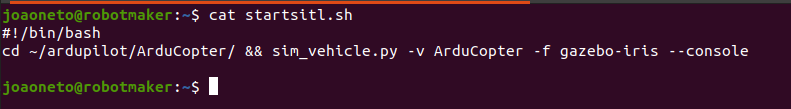
\includegraphics[width=0.8\textwidth]{Images/Desenvolvimento/startsitl.sh.png}
  \caption{startsitl.sh com Gazebo}
  \label{fig:startsitl_nogazebo.png.0}
\end{figure}
%

O modelo de mundo 3D utilizado no Gazebo para a integração com o SITL foi obtido a partir do repositorio de un canal do \textit{Youtube} chamado \cite{url:iq}. 
%
\begin{figure}[H]
  \centering
  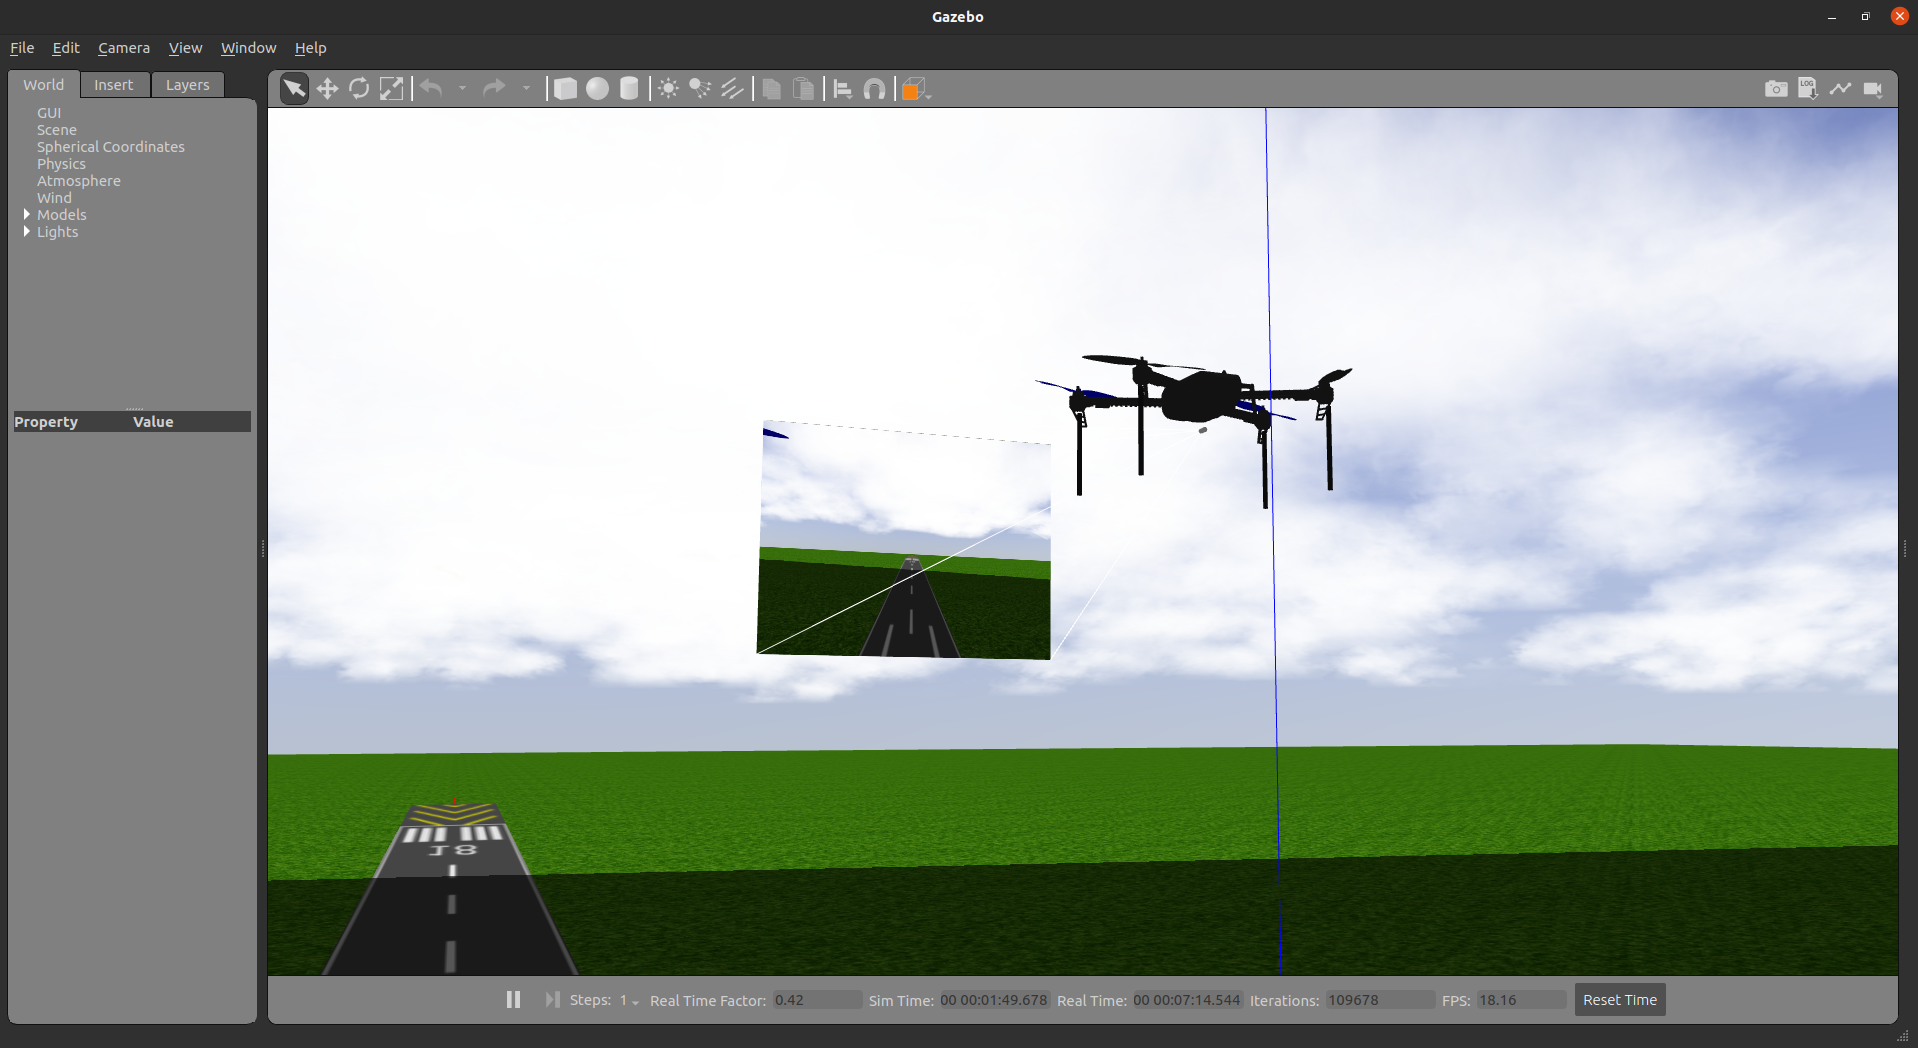
\includegraphics[width=0.7\textwidth]{Images/Desenvolvimento/sitl_gazebo.png}
  \caption{\textit{Software In The Loop} com Gazebo}
  \label{fig:sitl_gazebo.png.0}
\end{figure}
%
Essa instância do Gazebo é iniciada a partir de um nó do ROS, que é executado com o comando da figura \ref{fig:ros_gazebo.png.0}.
%
\begin{figure}[H]
  \centering
  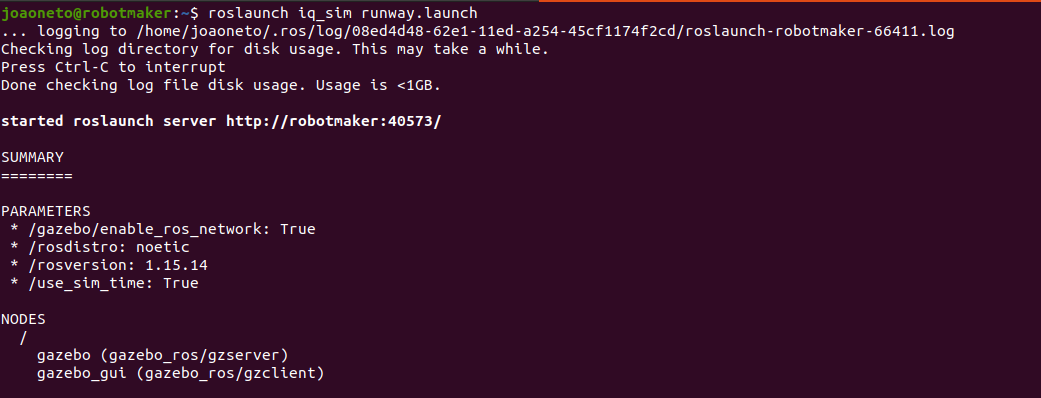
\includegraphics[width=0.7\textwidth]{Images/Desenvolvimento/ros_gazebo.png}
  \caption{Nó do Gazebo - ROS}
  \label{fig:ros_gazebo.png.0}
\end{figure}
%

Com isso, obtemos um ambiente de teste de desenvolvimento para as aplicações que sucederão. Os benefícios de se utilizar um ambiente de simulação como este é que não colocamos em risco o equipamento de hardware, nem as pessoas que seriam envolvidas em testes de campo. Além disso, o teste no ambiente computacional se torna mais prático, descartando toda a logística necessária para se deslocar com todo o equipamento para um campo aberto e com baixa densidade populacional.

O processo de instalação do ambiente de desenvolvimento do \textit{ArduPilot} está bem documentado nos apêndices deste documento, nesse processo também está incluído a instalação de dependências para executar o ambiente de simulação. 

\section{Ambiente de Simulação com o \textit{MAVROS}}

O \textit{MAVROS} como dito na parte introdutória, é um nó de ROS que publica e subscreve dados da controladora de voo, essas mensagens são trocadas utilizando o protocolo \textit{MAVlink}. O \textit{MAVROS} é geralmente configurado para realizar a comunicação através de um dispositivo serial, que no linux é identificado por um arquivo no diretório /dev. Entretanto, para fazer o \textit{MAVROS} se comunicar com o SITL, deve-se fazer uma modificação no arquivo de inicialização, arquivo com extensão \textit{.launch} no diretório launch do pacote.

No diretório launch do pacote são observados vários arquivos \textit{.launch} utilizados para iniciar o nó do \textit{MAVROS} com diferentes parâmetros. O apm.launch foi modificado como indicado na figura \ref{fig:mavros_launch.png.0}, para utilizar a porta de rede específica do \textit{MAVProxy} no SITL e não o dispositivo serial, comentado na linha superior.
%
\begin{figure}[H]
  \centering
  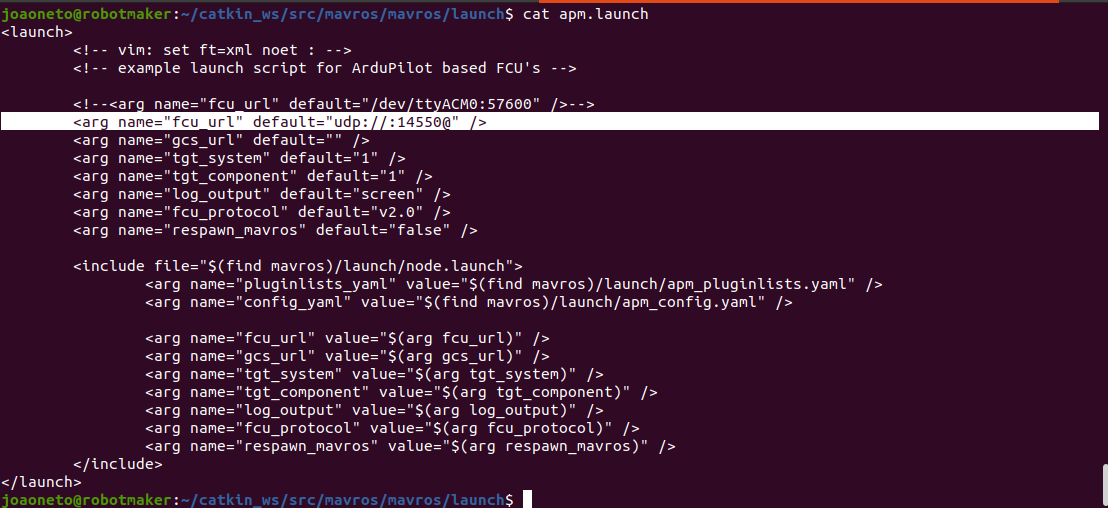
\includegraphics[width=0.7\textwidth]{Images/Desenvolvimento/mavros_launch.png}
  \caption{apm.launch do Pacote \textit{MAVROS}}
  \label{fig:mavros_launch.png.0}
\end{figure}
%
Com essa modificação, o nó do \textit{MAVROS} pode ser iniciado normalmente em conjunto com o SITL e é possível subscrever e publicar mensagens \textit{MAVlink} nos tópicos para a controladora de voo no ambiente simulado. 
%
\begin{figure}[H]
  \centering
  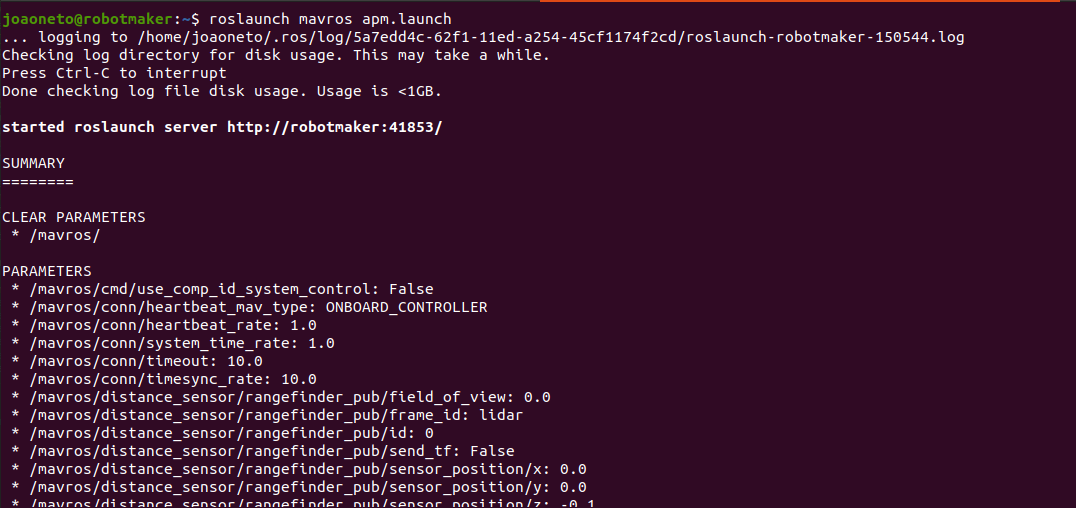
\includegraphics[width=0.7\textwidth]{Images/Desenvolvimento/mavros_execution.png}
  \caption{Execução do \textit{MAVROS}}
  \label{fig:mavros_execution.png.0}
\end{figure}
%
Alguns dos tópicos providos pelo \textit{MAVROS} são listados pelo comando rostopic list na figura \ref{fig:mavros_rostopic_list.png.0}. 
%
\begin{figure}[H]
  \centering
  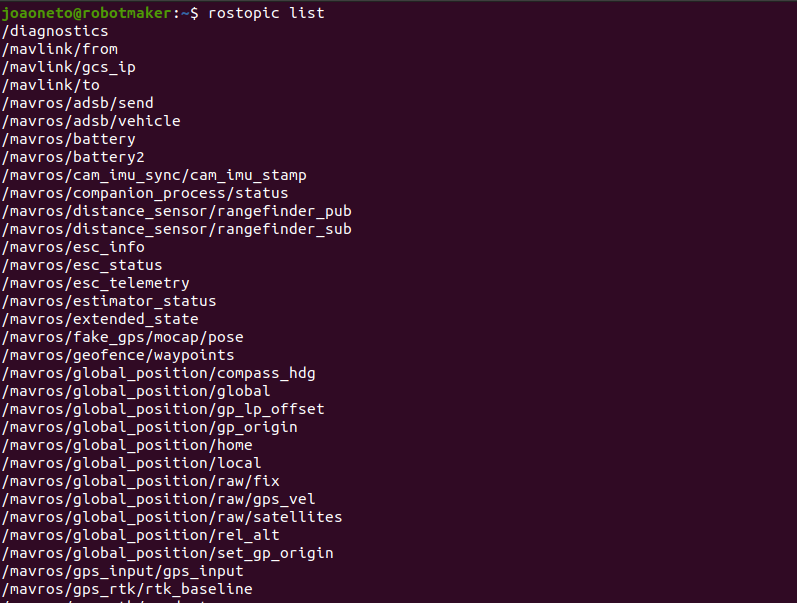
\includegraphics[width=0.7\textwidth]{Images/Desenvolvimento/mavros_rostopic_list.png}
  \caption{Tópicos do \textit{MAVROS}}
  \label{fig:mavros_rostopic_list.png.0}
\end{figure}
%
Por exemplo, o tópico correspondente a localização GPS da controladora de voo é o global\_position. É possível subscrever e acompanhar as mensagens que chegam da controladora nesse tópico pelo comando da figura \ref{fig:mavros_rostopic_echo.png.0}.
%
\begin{figure}[H]
  \centering
  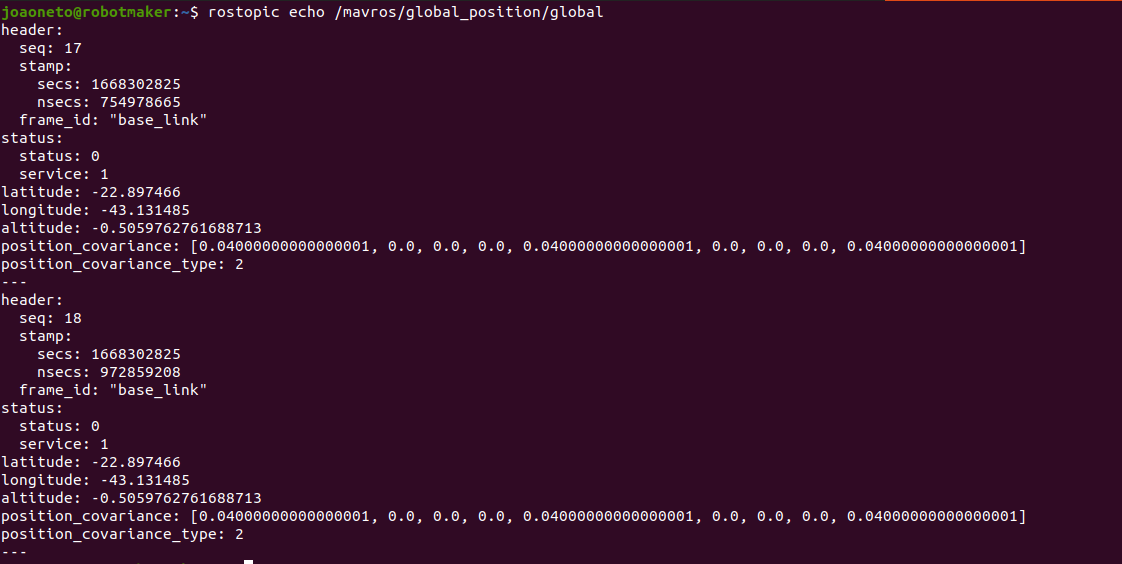
\includegraphics[width=0.7\textwidth]{Images/Desenvolvimento/mavros_rostopic_echo.png}
  \caption{Tópicos do \textit{MAVROS}}
  \label{fig:mavros_rostopic_echo.png.0}
\end{figure}
%

Os tópicos do ROS são facilmente acessados através de linguagens de programação como C++ e Python. Em particular esta última, possui um módulo chamado rospy que permite a criação de aplicações do ROS, com este módulo é possível desenvolver nós inteiramente usando Python. Com o \textit{MAVROS} agindo como uma interface da aeronave, é possível desenvolver um nó que se comunique com ele e também com a API em Django.

\section{Arquitetura da aplicação embarcada}

Inicialmente, houve-se uma ideia de fazer um pacote com um nó apenas agregando tanto funcionalidades de telemetria quanto de controle. Entretanto, para facilitar o desenvolvimento e trazer a opção de utilização de cada funcionalidade separadamente, optou-se por dividir as funcionalidades em dois nós distintos.  

Os programas que são executados no computador de bordo para executar a aplicação, são os listados abaixo: 
\begin{enumerate}
  \item \textit{MAVProxy} [\textit{script Python} disponibilizado pela comunidade]
  \item \textit{MAVROS} [\textit{Pacote} do \textit{ROS} disponibilizado pela comunidade]
  \item \textit{drone\_telemetry\_over\_network} [\textit{Pacote} do \textit{ROS} autoral]
  \item \textit{drone\_control\_over\_network} [\textit{Pacote} do \textit{ROS} autoral]
\end{enumerate}

Além desses programas, um pacote do \textit{ROS} chamado \textit{iq\_gnc} disponibilizado pelo canal \cite{url:iq}, foi utilizado como dependência, por conter funções de comunicação com o \textit{MAVROS} muito úteis para o desenvolvimento dos nós de comunicação. Entretanto, ao longo do desenvolvimento esse pacote precisou ser expandido para um maior número de funções.

\subsection{\textit{drone\_telemetry\_over\_network}}

O pacote do \textit{ROS}, \textit{drone\_telemetry\_over\_network}, foi criado para conter todas as funcionalidades de telemetria do \textit{drone}. Nesse pacote foi desenvolvido um \textit{script} com o nome \textbf{\textit{telemetry\_node.py}} que é o nó responsável por subscrever nos tópicos do \textit{MAVROS}, receber as mensagens publicadas pela controladora nesses tópicos e enviá-las num formato \textit{JSON} para a API. Além disso, outras informações do próprio computador de bordo, como endereço de IP, uso de memória e uso de CPU foram incluídas nessas mensagens.

A partir do diagrama abaixo podemos ver como o nó de telemetria (\textit{telemetry\_node.py}) foi implementado:
%
\begin{figure}[H]
  \centering
  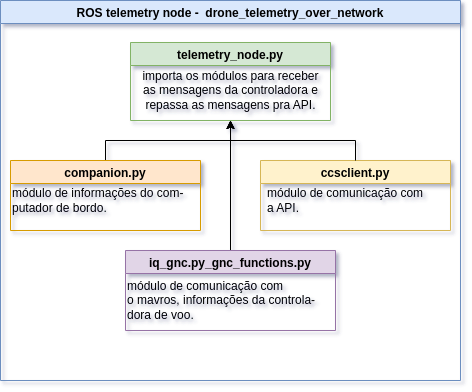
\includegraphics[width=0.6\textwidth]{Images/Desenvolvimento/telemetry_arq.png}
  \caption{Arquitetura do nó de telemetria.}
  \label{fig:telemetry_arq.png.0}
\end{figure}
%

O módulo \textbf{\textit{companion.py}} possui diversas funções que permitem coletar o estado do computador de bordo, as informações coletadas são: força do sinal \textit{Wi-Fi} recebido, nome da interface de rede \textit{Wi-Fi}, \textit{IP} local e público, recursos totais e consumidos de memória física, memória virtual e \textit{CPU}, além dessas também são coletadas informações do sistema como o nome do sistema operacional que no caso é Ubuntu, versão do sistema operacional, arquitetura do processador, hostname de rede e a lista de todos os processos sendo executados no momento.  

O pacote \textbf{\textit{iq\_gnc}} foi importado para abstrair a comunicação com o \textit{MAVROS}, neste pacote existem inúmeras funções que permitem a programação da telemetria e controle do drone em um nível mais alto do que seria possível utilizando diretamente os módulos \textit{mavros\_msgs} e \textit{rospy}.

O nó utiliza \textit{websockets} para se comunicar com a API e por conta disso foi desenvolvido um módulo de \textit{Python}, chamado de \textbf{\textit{ccsclient.py}} para encapsular as funcionalidades de comunicação e com isso abstrair o código necessário para enviar mensagens de telemetria à API. Tais mensagens, por sua vez, possuem uma estrutura predefinida para que a aplicação WEB possa importá-la corretamente. Um exemplo de mensagem de telemetria pode ser visto a seguir:

\begin{lstlisting}[
language=Python,
basicstyle=\tiny, %or \small or \footnotesize etc.
]
{
  "type": "telemetry",
  "message": {
    "companion": {
      "system": {
        "config": {
          "system": "Linux",
          "node_name": "robotmaker",
          "release": "5.15.0-50-generic",
          "version": "#56~20.04.1-Ubuntu SMP Tue Sep 27 15:51:29 UTC 2022",
          "machine": "x86_64",
          "processor": "x86_64"
        },
        "platform": {
          "cpu_percent": 83.7,
          "virtual_memory": {
            "total": 16494366720,
            "available": 11268907008,
            "percent": 31.7,
            "used": 3923206144,
            "free": 6610907136,
            "active": 2248499200,
            "inactive": 5946028032,
            "buffers": 434647040,
            "cached": 5525606400,
            "shared": 965926912,
            "slab": 728702976
          },
          "virtual_memory_available": 68.31973121063238,
          "virtual_memory_used": 31.7
        },
        "processes": [
          {
            "name": "chrome",
            "pid": 9971,
            "username": "joaoneto",
            "vms": 1156966.5
          },
          {
            "name": "chrome",
            "pid": 9780,
            "username": "joaoneto",
            "vms": 1156554.1875
          }
        ]
      },
      "connectivity": {
        "rssi": [
          [
            "wlp2",
            "-53"
          ]
        ],
        "local_ip": "192.168.1.173",
        "public_ip": "179.218.3.60"
      }
    },
    "state": {
      "connected": true,
      "armed": false,
      "guided": false,
      "manual_input": true,
      "mode": "STABILIZE",
      "system_status": 3
    },
    "position": {
      "location": {
        "x": -0.008386431068842331,
        "y": 0.012552853294305917,
        "z": -0.071,
        "theta": 1.366358710597936
      },
      "gps": {
        "long": -43.1314851,
        "lat": -22.8974658
      }
    }
  }
}
\end{lstlisting}


Com o \textit{script} do \textit{SITL} iniciado e o \textit{MAVROS} em execução, o nó de telemetria desenvolvido pode ser iniciado a partir de um comando do \textit{ROS} como demonstrado na figura abaixo:
%
\begin{figure}[H]
  \centering
  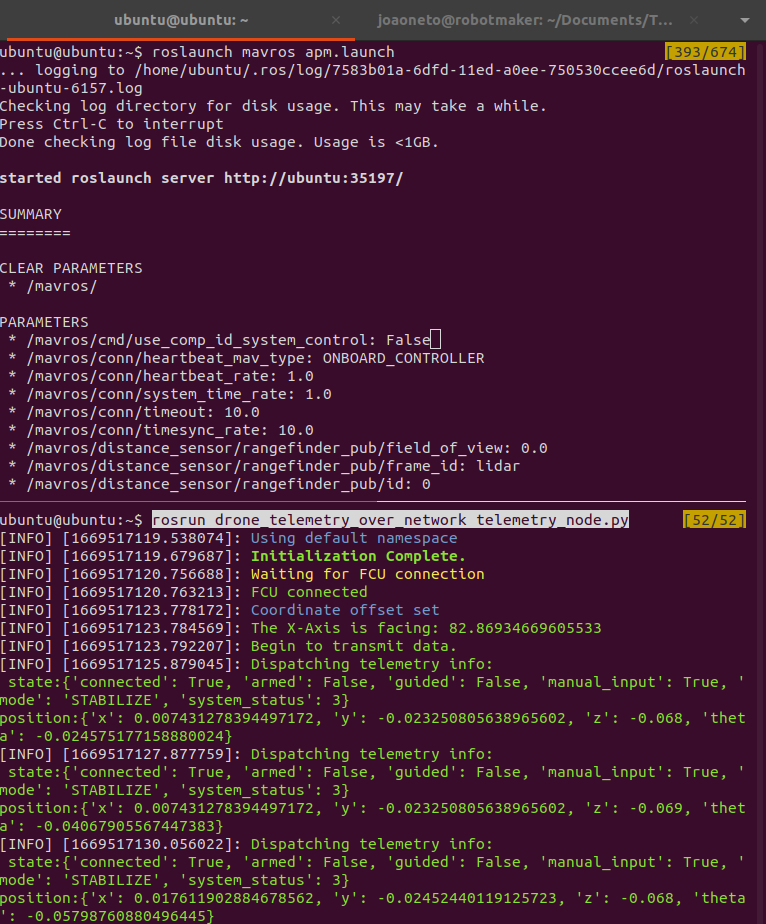
\includegraphics[width=0.7\textwidth]{Images/Desenvolvimento/telemetry_node.png}
  \caption{\textit{MAVROS} e nó de telemetria em execução.}
  \label{fig:telemetry_node.png.0}
\end{figure}
%


\subsection{\textit{drone\_control\_over\_network}}

O pacote do \textit{ROS}, \textit{drone}\_control\_over\_network, desenvolvido posteriormente, herdou muitas características do pacote de telemetria. Entretanto, esse pacote contém o \textit{script} \textbf{\textit{control\_node.py}} que é o nó responsável por fazer o caminho de comunicação inverso do seu antecessor, isto é, receber comandos da \textit{API} e publicar as mensagens nos tópicos do \textit{MAVROS}, permitindo assim o controle do \textit{drone} através da aplicação \textit{WEB}. Segue na figura \ref{fig:comm_nodes.png.0} os dois pacotes de comunicação lado a lado.

%
\begin{figure}[H]
  \centering
  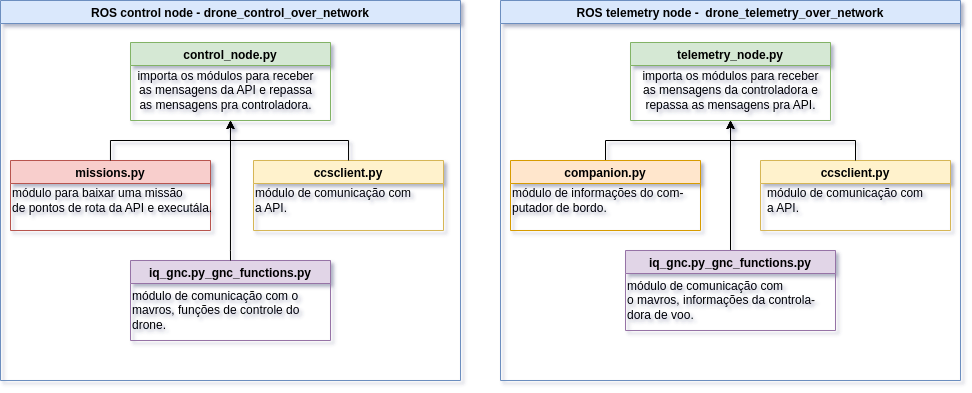
\includegraphics[width=1\textwidth]{Images/Desenvolvimento/comm_nodes.png}
  \caption{Comparação dos pacotes de comunicação.}
  \label{fig:comm_nodes.png.0}
\end{figure}
%

O nó de controle utiliza os mesmos módulos, \textit{ccsclient.py} e \textit{iq\_gnc.py} do pacote de telemetria, entretanto não utiliza o módulo \textit{companion.py} e importa um outro módulo: \textit{missions.py} que implementa a funcionalidade de carregamento de missões de pontos de rota. Esta funcionalidade serve para que o \textit{drone} baixe e interprete um arquivo de missão, que é um arquivo de texto em que cada linha significa um ponto de rota diferente com coordenadas específicas. O padrão de arquivo de missão utilizado vem do programa \textit{QGroundControl}, e desenvolvido pela comunidade ArduPilot, um exemplo de arquivo pode ser visualizado na figura \ref{fig:qgcwpl.png.0}.
%
\begin{figure}[!htbp]
  \centering
  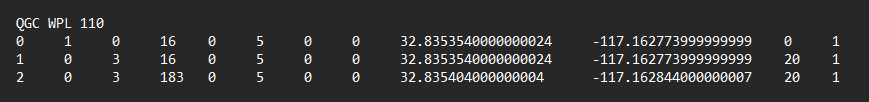
\includegraphics[width=0.8\textwidth]{Images/Desenvolvimento/qgcwpl.png}
  \caption{Exemplo de arquivo de missão.}
  \label{fig:qgcwpl.png.0}
\end{figure}
%

A mensagem de controle que o usuário manda através da aplicação \textit{WEB} também tem um formato específico e é exemplificada abaixo. Tal mensagem é lida pelo nó de controle e então é traduzida em uma das funções pré-programadas do módulo \textit{iq\_gnc}, que é utilizado para publicar a mensagem em algum tópico do \textit{mavros} e então comandar o \textit{drone}. 

\begin{lstlisting}[
language=Python,
basicstyle=\tiny, %or \small or \footnotesize etc.
]
{
  "type": "control",
  "message": {
    "control_echo": false,
    "command": {
      "function": {
        "name": "<COMMAND_NAME>",
        "params": "<PARAMETER>"
      }
    }
  }
}
\end{lstlisting}
Após executar a função, o nó responde com uma mensagem de \textit{flag control\_echo = true} para a aplicação \textit{WEB}, contendo algumas informações sobre o resultado da execução. A figura \ref{fig:control_node.png.0} mostra \textit{mavros}, nó de telemetria e nó de controle sendo executados no mesmo terminal. 
%
\begin{figure}[!htbp]
  \centering
  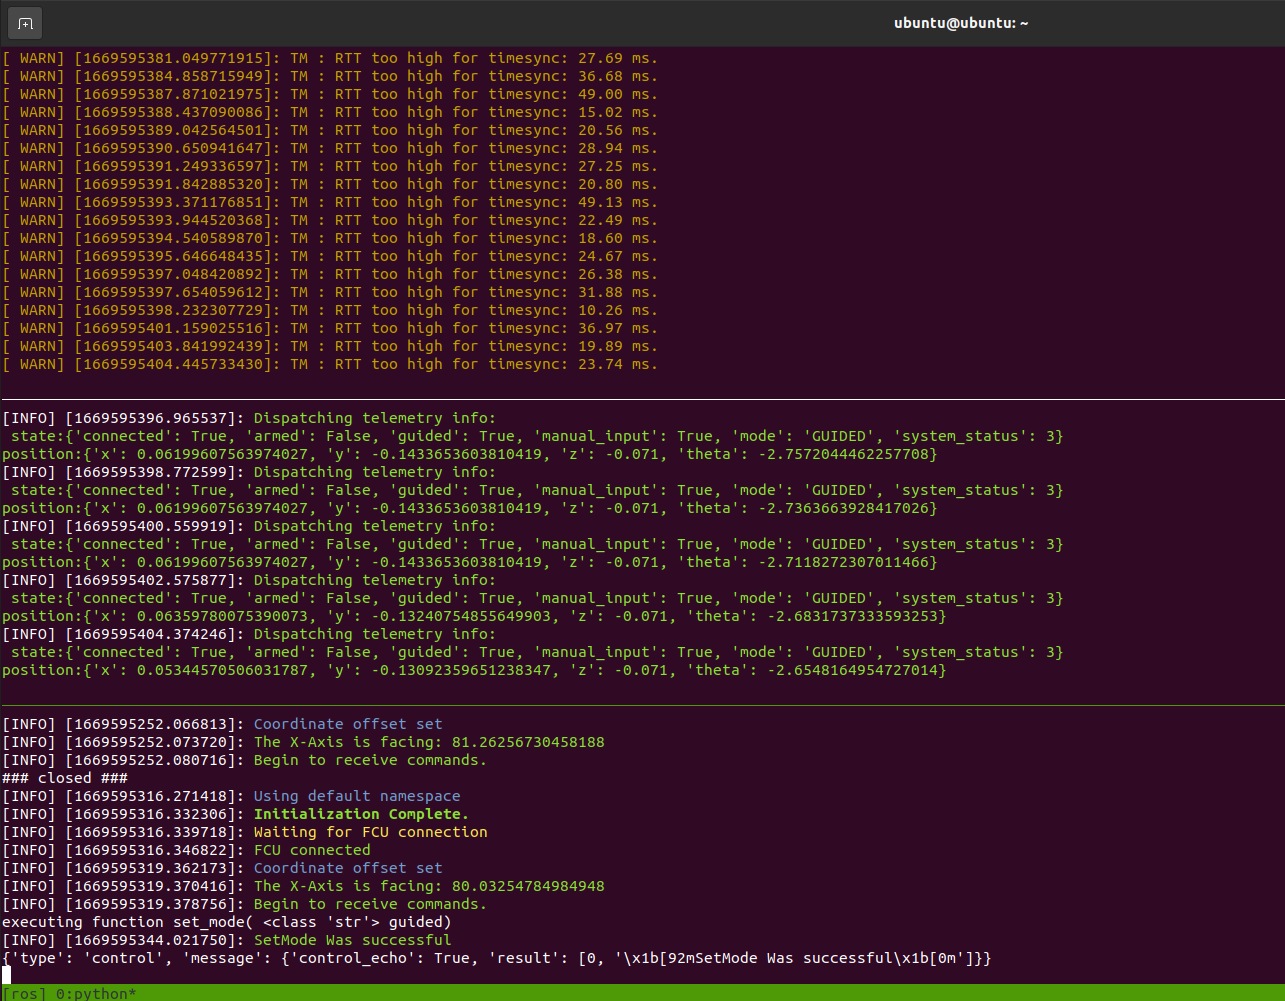
\includegraphics[width=0.7\textwidth]{Images/Desenvolvimento/control_node.png}
  \caption{Execução do \textit{mavros, telemetry\_node.py} e \textit{control\_node.py} respectivamente.}
  \label{fig:control_node.png.0}
\end{figure}
%

\section{Arquitetura da \textit{Cloud Control Station - CCS}}

A \textit{CCS} foi inicialmente concebida apenas como uma \textit{API} utilizando o \textit{Django Rest Framework}, a ideia era utilizar requisições \textit{http} tanto do lado do usuário quanto do lado do computador de bordo. Entretanto, no processo de pesquisa evidenciou-se que para aplicações onde a comunicação é bidirecional a utilização de \textit{websockets} seria a melhor opção. De fato, para aplicações \textit{WEB} em tempo real, o processo de requisição e resposta \textit{HTTP} não é compatível com a necessidade de atualização de conteúdo imediato demandada pelo cliente, visto que para que isso ocorra o cliente precisa requerer a todo momento por atualizações do servidor, o que em escala torna-se muito oneroso para a aplicação. Por outro lado, a aplicação com \textit{websockets} possibilita a criação de uma conexão entre as partes e uma abordagem mais orientada a eventos, no qual a partir do evento de uma nova mensagem ela é imediatamente consumida por uma das partes.

%
\begin{figure}[H]
  \centering
  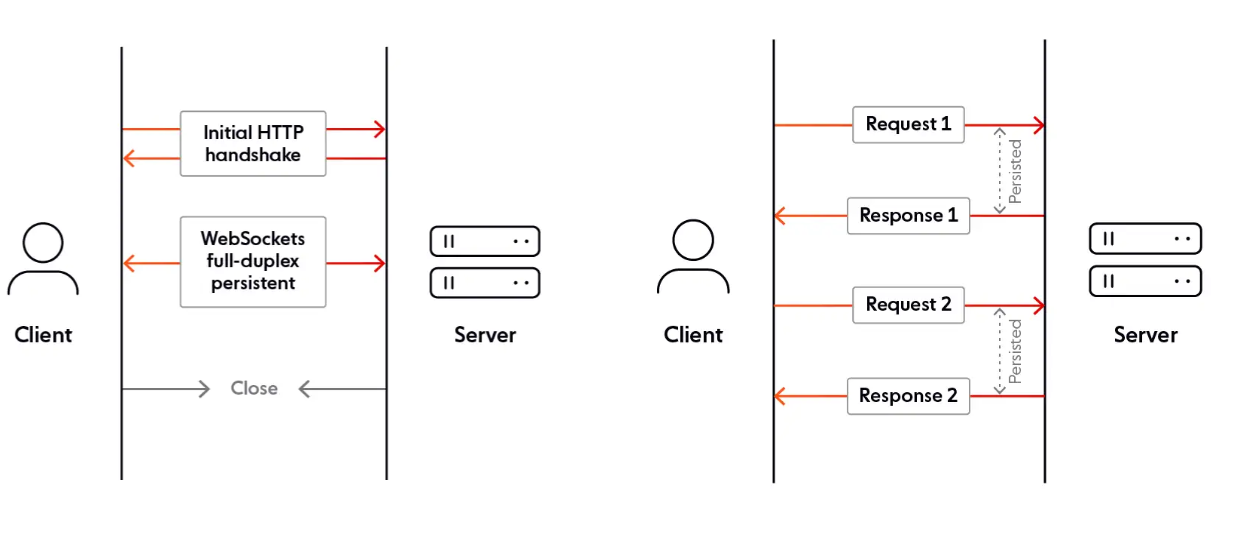
\includegraphics[width=0.7\textwidth]{Images/Diagramas/http-long-polling.png}
  \caption{Comparação entre o \textit{HTTP} e o \textit{Websocket}.(FONTE~\cite{url:websocket_vs_http})}
  \label{fig:http-long-polling.png.0}
\end{figure}
%

Seguindo esse princípio, foi determinado que a aplicação \textit{WEB} trabalharia com os dois protocolos ao mesmo tempo. Para isso, o módulo \textit{Django Channels} foi utilizado para implementar a comunicação via \textit{websockets} e o módulo \textit{Django REST Framework} foi destinado para as funcionalidades de \textit{API REST} utilizando o protocolo \textit{HTTP}.

%
\begin{figure}[H]
  \centering
  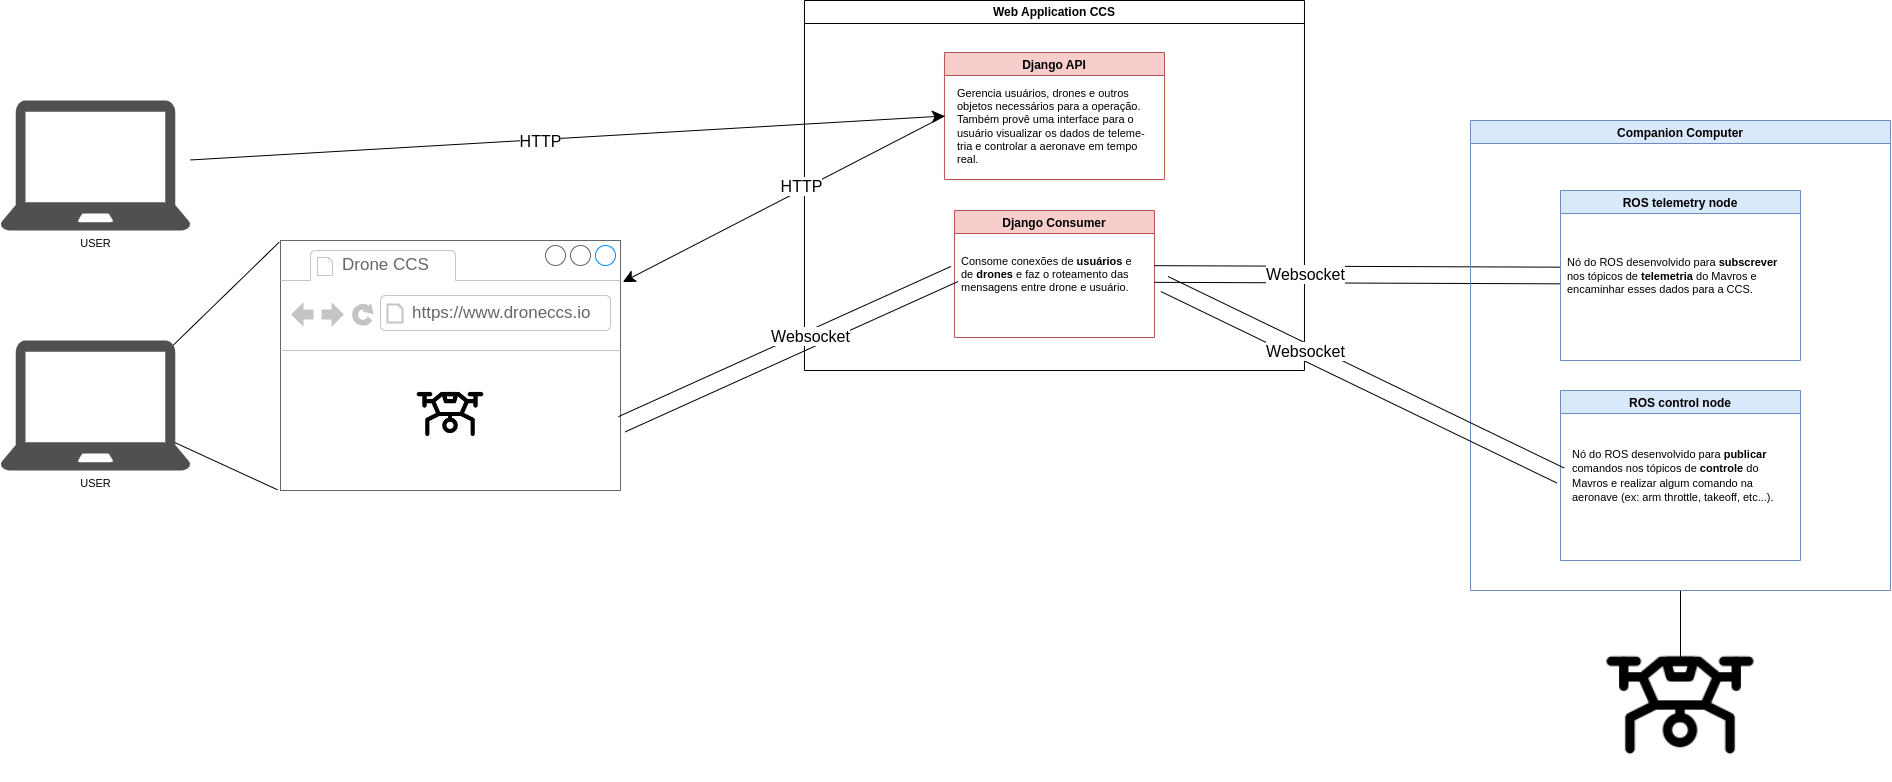
\includegraphics[width=1\textwidth]{Images/Diagramas/CCS_protocol_ARQ.png}
  \caption{Diagrama de protocolos de aplicação utilizados na \textit{CCS}.}
  \label{fig:CCS_protocol_ARQ.png.0}
\end{figure}
%

Como demonstrado na figura \ref{fig:CCS_protocol_ARQ.png.0}, o \textit{HTTP} é utilizado pelo usuário inicialmente para requisitar uma página \textit{WEB}, que por sua vez possui um código em \textit{JavaScript} que inicia uma conexão \textit{Websocket} com a aplicação. Do outro lado da comunicação, o computador de bordo inicia duas conexões via \textit{websockets}, uma para cada nó de comunicação. O fluxo de comunicação descrito é a funcionalidade principal do sistema desenvolvido. Outras funcionalidades e detalhes da aplicação serão discutidos nas próximas seções.

\newpage

\subsection{Autenticação}

Para garantir o mínimo de segurança para a aplicação desenvolvida, que poderá ser disponibilizada na \textit{Internet}, foram implementados alguns métodos de autenticação utilizando os módulos já disponíveis no \textit{Django}. Para o protocolo HTTP são suportados 3 métodos de autenticação diferentes, são eles:
\begin{itemize}
    \item Autenticação via \textit{JWT (JSON Web Token)} para o usuário. 
    \item Autenticação via chave de \textit{API} para o \textit{drone}.
    \item Autenticação via chave de sessão para o usuário (necessário para utilização da interface do \textit{Django REST Framework}). 
\end{itemize}

Para que o usuário consiga chamar a maior parte dos métodos da \textit{API} ele deve estar autenticado por um dos métodos mencionados acima. Obviamente, o único método que não necessita de autenticação é o método de registro de usuário. A figura \ref{fig:regster_user.png.0} exemplifica o registro do usuário feito através de interface padrão do \textit{Django REST Framework}.
%
\begin{figure}[!htbp]
  \centering
  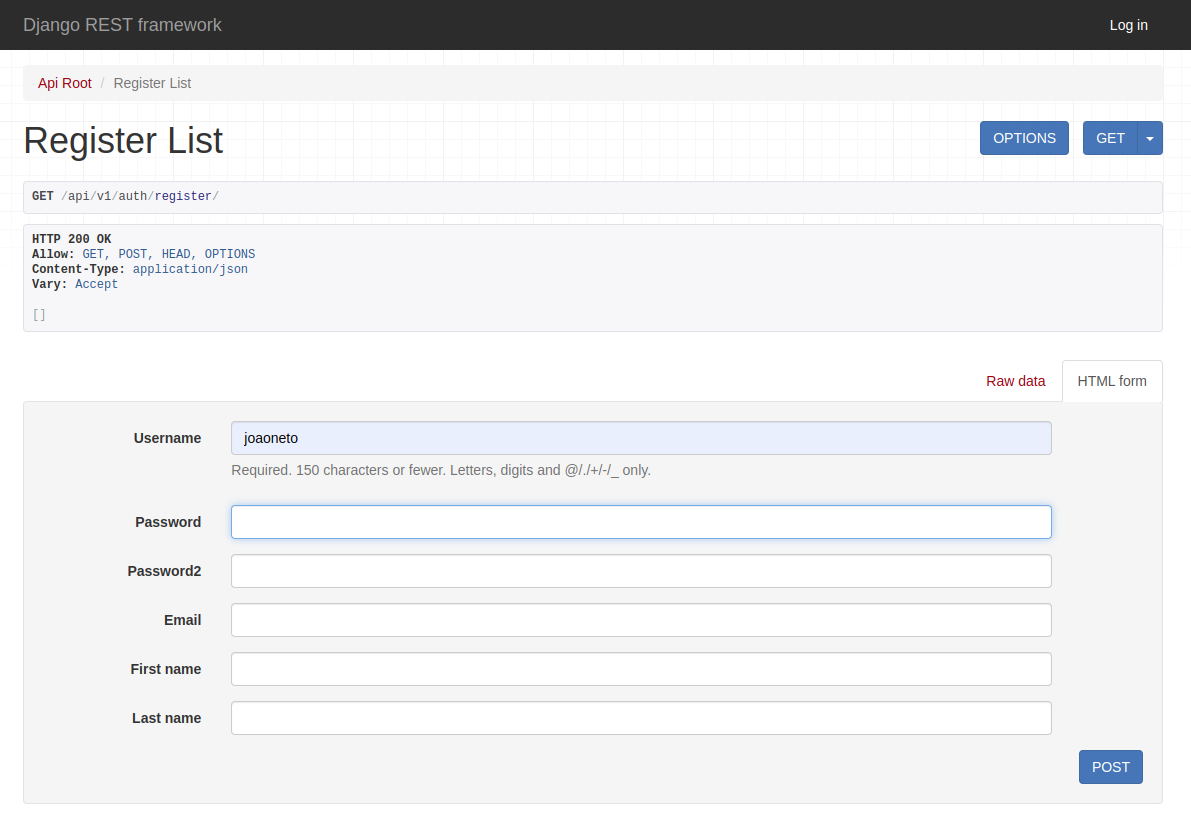
\includegraphics[width=0.7\textwidth]{Images/Desenvolvimento/register_user.png}
  \caption{Tela para registro de usuário.}
  \label{fig:regster_user.png.0}
\end{figure}
%
Após criar o usuário e logar com o mesmo, é possível acessar o método de \textit{API} para o registro de um novo \textit{drone} associado a esse usuário. 
%
\begin{figure}[!htbp]
  \centering
  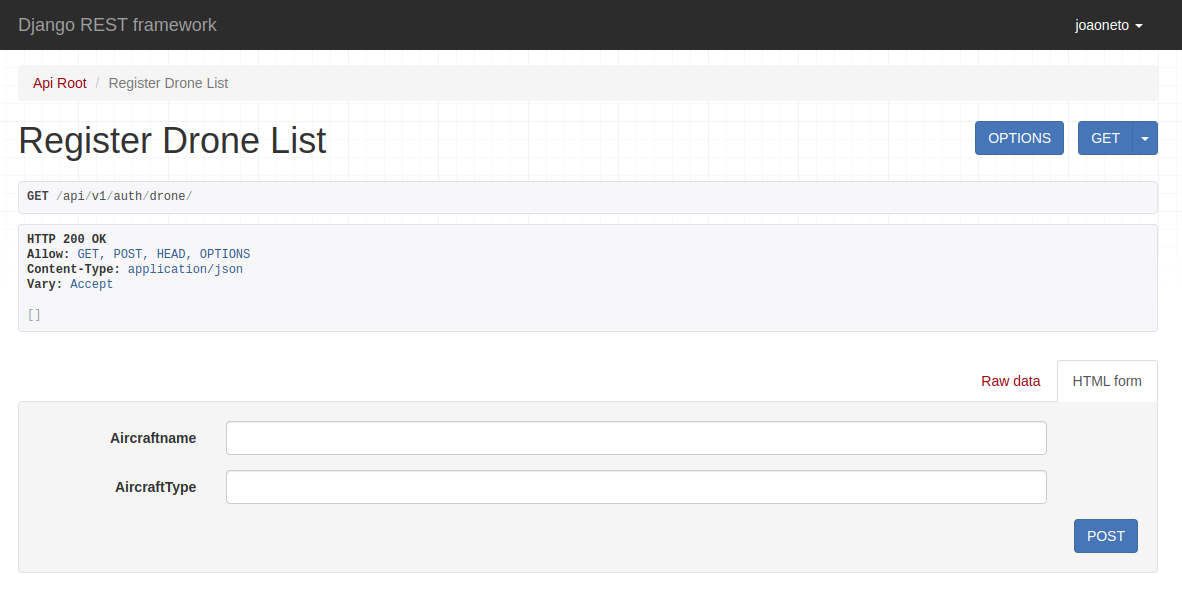
\includegraphics[width=0.7\textwidth]{Images/Desenvolvimento/drone_register.png}
  \caption{Tela para registro do \textit{drone}.}
  \label{fig:drone_register.png.0}
\end{figure}
%
%
\begin{figure}[!htbp]
  \centering
  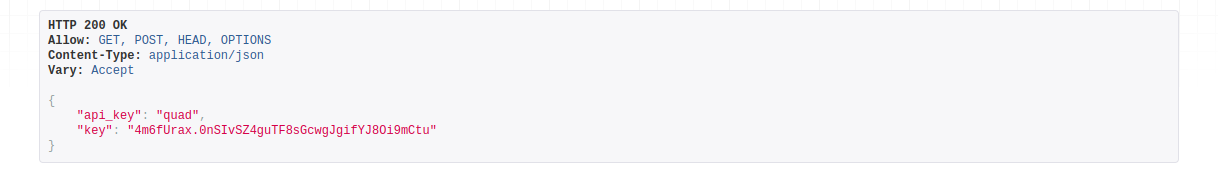
\includegraphics[width=0.7\textwidth]{Images/Desenvolvimento/register_drone_resp.png}
  \caption{Resposta do registro do \textit{drone}.}
  \label{fig:register_drone_resp.png.0}
\end{figure}
%
Com o registro do \textit{drone}, é gerada uma chave de \textit{API} que deverá ser instalada como uma variável de ambiente no computador de bordo do \textit{drone}. Além da chave de \textit{API} o nome da aeronave e o domínio da \textit{API} devem ser especificados como variáveis de ambiente, para persistência dessas variáveis utilizou-se o arquivo .profile no diretório /home do usuário.
%
\begin{figure}[!htbp]
  \centering
  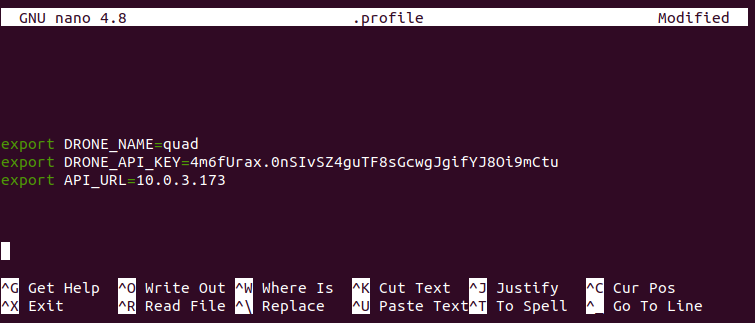
\includegraphics[width=0.7\textwidth]{Images/Desenvolvimento/drone_api_key.png}
  \caption{Instalação da chave de \textit{API} no \textit{drone}.}
  \label{fig:drone_api_key.png.0}
\end{figure}
%
\subsection{Funcionalidades}

\subsubsection{Gerenciamento de usuários}

\subsubsection{Gerenciamento de aeronaves}

\subsubsection{Gerenciamento de missões}

\subsubsection{Funções de controle e telemetria}


\section{Outras arquiteturas possíveis para o sistema proposto}

LTE e 5G.

\section{Primeiros testes com o \textit{drone} quadricóptero}

De posse de um \textit{drone} quadricóptero com a controladora de voo \textit{Omnibus f4 pro}, foram estabelecidos os primeiros testes de conexão entre o \textit{Raspberry Pi} e o \textit{firmware ArduPilot}. O diagrama de montagem do equipamento foi o seguinte:

\subsection{Diagrama de conexão dos componentes de hardware}
%
\begin{figure}[!htbp]
  \centering
  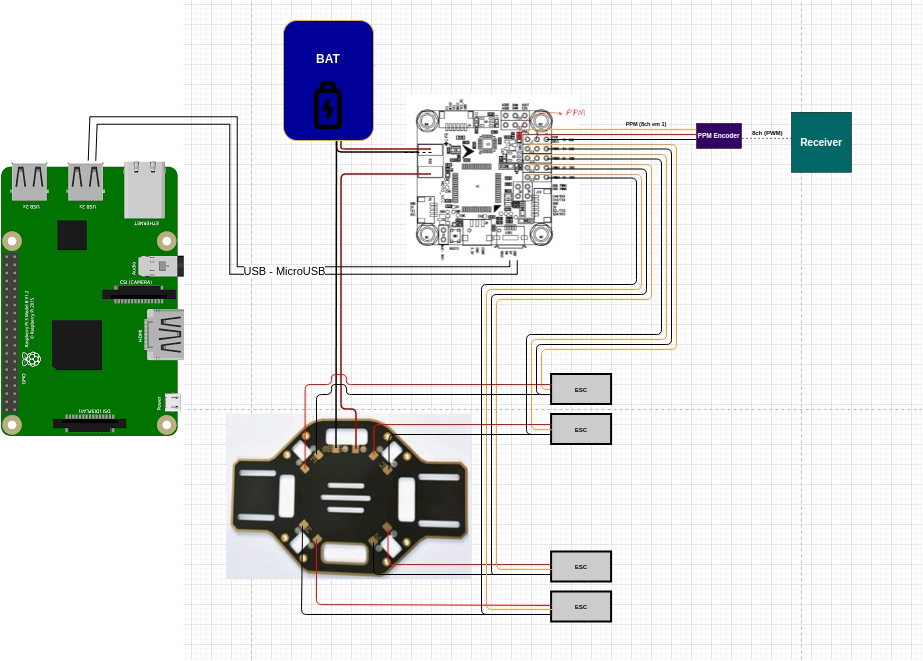
\includegraphics[width=0.7\textwidth]{Images/Diagramas/hardware_connections.png}
  \caption{Conexões de hardware para Omnibus F4 Pro V3.}
  \label{fig:hardware_connections.png.0}
\end{figure}
%
A motivação para a escolha dessa controladora foi o preço dela no mercado em relação às outras, valor que na época era em torno de 260 reais, enquanto que a Pixhawk custava em torno de 1000 reais. O resto dos componentes também foi escolhido com o intuito de deixar o projeto em baixo custo. 
%

Após a ligação dos componentes eletrônicos, o teste de conexão entre o Raspberry e a controladora foi realizado utilizando o \textit{software MAVProxy} no minicomputador e foi possível obter dados em tempo real da controladora através da conexão serial assim como também foi possível mandar comandos \textit{MAVlink} para a controladora de voo através do terminal da aplicação.

%
\begin{figure}[!htbp]
  \centering
  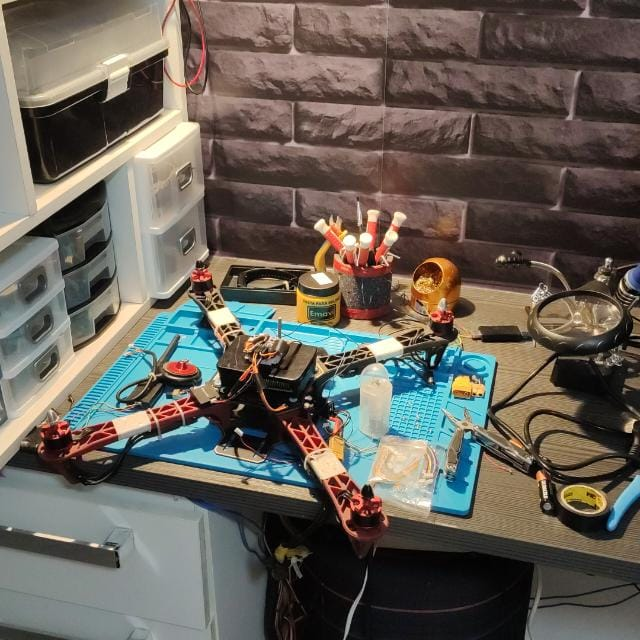
\includegraphics[width=0.7\textwidth]{Images/Desenvolvimento/omnibus_drone.jpeg}
  \caption{Bancada de trabalho com o \textit{drone} quadricóptero.}
  \label{fig:omnibus_drone.jpeg.0}
\end{figure}
%
Dessa forma, conseguiu-se comandar o \textit{drone} a partir do computador de bordo e receber dados de telemetria dele. Entretanto, não foi possível acoplar o módulo de GPS na controladora já que o módulo em questão não se mostrou compatível com ela.

As pesquisas e soluções de problemas oriundos da execução dessa etapa foram cruciais para adquirir maturidade na montagem, configuração e acoplamento dos componentes. Além disso, o conhecimento adquirido das ferramentas utilizadas para conectar o computador de bordo ao \textit{drone} também foram essenciais. Entretanto, escolhemos mudar o hardware utilizado para uma configuração de \textit{drone} mais convencional na comunidade \textit{ArduPilot}, com a controladora Pixhawk Cube. 

\section{Montagem do \textit{drone} hexacóptero}

Após os problemas obtidos no \textit{drone} quadcóptero com a controladora Omnibus, trocamos o hardware utilizado para um \textit{drone} hexacóptero com a controladora Pixhawk Cube. Tal aeronave já estava operacional antes de acoplarmos o Raspberrypi, isto é, era possível realizar todas as funções básicas que a controladora por si só é capaz de fazer.
%
\begin{figure}[!htbp]
  \centering
  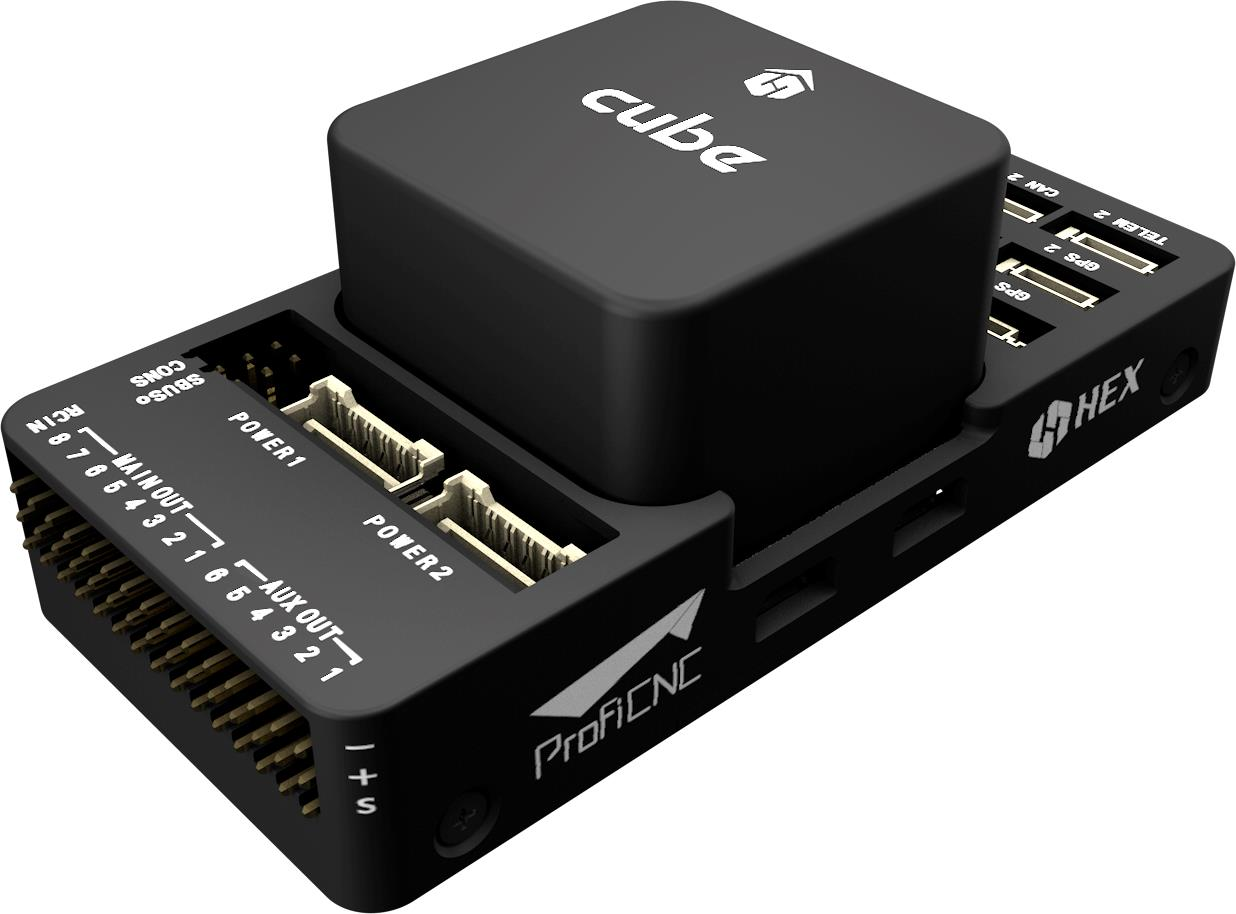
\includegraphics[width=0.4\textwidth]{Images/Desenvolvimento/pixhawk2_cube_hero.png}
  \caption{Pixhawk 2 Cube Hero.}
  \label{fig:pixhawk2_cube_hero.png.0}
\end{figure}
%

Com isso, obtemos a seguinte conexão dos componentes:
\subsection{Diagrama de conexão dos componentes de hardware}
%
\begin{figure}[!htbp]
  \centering
  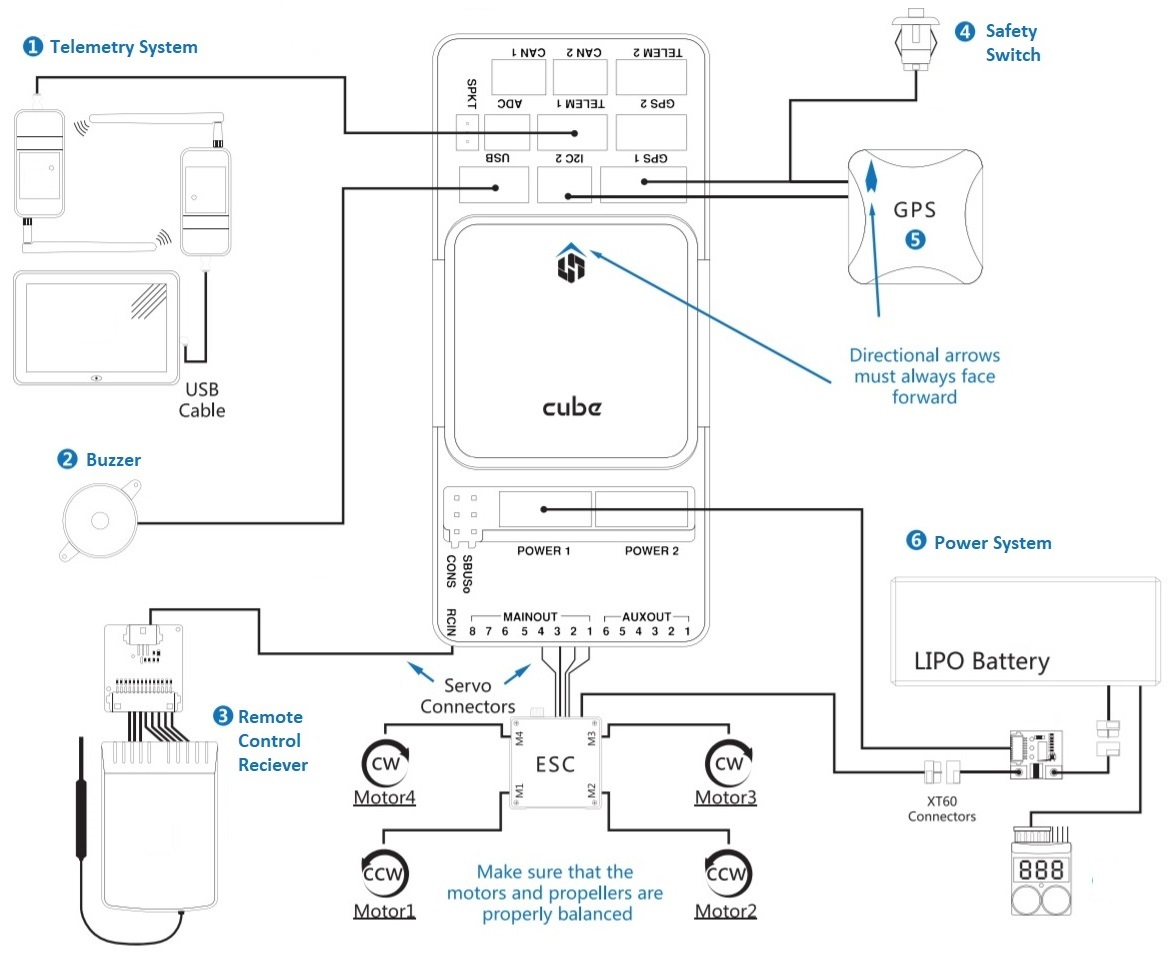
\includegraphics[width=0.7\textwidth]{Images/Diagramas/cube_wiring_overview.jpg}
  \caption{Conexões de hardware para a Pixhawk 2 Cube Hero.}
  \label{fig:cube_wiring_overview.jpg.0}
\end{figure}
%

<motivação da escolha desse hardware>
<características desse hardware>
<capacidades desse \textit{drone}>

<conseguir mais fotos do \textit{drone}>
<mostrar ligação dos componentes e tudo funcionando perfeitamente>
<motivação da escolha desse hardware>
<características desse hardware>
<capacidades desse \textit{drone}>

\newpage

\chapter{Resultados}
%
% retira numeracao da pagina, conforme as normas de apresentacao.
\thispagestyle{empty} 
%
apresentação de resultados (numéricos e/ou gráficos) 
de cálculos e/ou de simulações, requeridos na especificação do trabalho.

%%%%%%%%%%%%%%%%%%%%%%%%%%%%%%%%%%%%%%%%%%%%%%%%%%%


%%%%%%%%%%%%%%%%%%%%%%%%%%%%%%%%%%%%%%%%%%%%%%%%%%%%%%%%
%                      Conclusão                       %
%%%%%%%%%%%%%%%%%%%%%%%%%%%%%%%%%%%%%%%%%%%%%%%%%%%%%%%%

\chapter{Conclusão}
%
% retira numeracao da pagina, conforme as normas de apresentacao.
\thispagestyle{empty} 
%

\hl{Hipótese testada
Se realizarmos o experimento em outro ambiente com maior capacidade para que todos possam assistir de forma homogênea atenderemos a demanda da turma, teremos um aprendizado mais efetivo e melhoria no tempo dedicado a esse experimento.

Responda as perguntas avaliativas para definir a conclusão}
\begin{enumerate}
    \item pergunta avaliativa 1
    \item pergunta avaliativa 2
    \item pergunta avaliativa 3
    \item pergunta avaliativa 4
\end{enumerate}

Esta monografia tem como base a pesquisa, a elaboração e o teste, em ambiente simulado, de um \textit{drone} capaz de se comunicar por uma rede IP, no nosso caso,
uma rede \textit{wi-fi}. 

Aproveitou-se conhecimentos adquiridos na equipe UFFO \cite{url:equipeuffo}, como \textit{softwares} e bibliotecas específicas para automação. A partir
dessa base, surgiu a ideia de incrementar o \textit{hardware} de um \textit{drone} comum acoplando um \textit{Raspberry}. A grande adição é o acesso ao protocolo IP, permitindo o \textit{drone} trocar dados sem limitações de distância. Para realizar a comunicação com o \textit{drone}, foi elaborada uma arquitetura de cliente-servidor, cujo cliente, em resumo o \textit{drone}, envia e recebe dados do servidor, ambos conectados numa mesma rede, via VPN. Por fim, realizou-se uma página \textit{web} como \textit{interface} gráfica final, a qual permite o envio de missões ao \textit{drone} e exibe os dados essenciais de telemetria em tempo real.  

No geral, os resultados foram compatíveis aos objetivos propostos, realizaram-se testes no ambiente de simulação que demonstraram a viabilidade de um projeto prático.  

O projeto como um todo ainda deve ser aperfeiçoado casa haja interesse em comercialização. Faz-se necessário a realização de testes com um \textit{drone} fora do ambiente de simulação, e como citado no Capítulo 1~\ref{item:solucao}, idealmente, conectar um modem LTE ou NR ao \textit{Raspberry}. Ambos, os testes e a conexão do modem, podem ser feitos por futuros integrantes da equipe UFFO.


%%%%%%%%%%%%%%%%%%%%%%%%%%%%%%%%%%%%%%%%%%%%%%%%%%%%%%%%
%          Sugestoes para trabalhos futuros            %
%%%%%%%%%%%%%%%%%%%%%%%%%%%%%%%%%%%%%%%%%%%%%%%%%%%%%%%%

\section{Sugestões para trabalhos futuros}
%
% retira numeracao da pagina, conforme as normas de apresentacao.
\thispagestyle{empty} 
%
%
Tendo em mente as características do projeto apresentadas neste trabalho, podemos imaginar diversas aplicações para serem acrescentadas. Somos capazes, portanto, de listar algumas das possíveis aplicações e seus possíveis desdobramentos.
%
\begin{enumerate}
    \item Melhorias na interface de controle 
        \begin{enumerate}
            \item Adição de novos funcionalidades
            \item Coleta e apresentação de mais dados do \textit{drone}  
        \end{enumerate}
    \item Integração de um modem de \textit{Internet} móvel
        \begin{enumerate}
            \item Controle e coleta de dados a qualquer distância, desde que haja sinal de \textit{Internet} móvel.
        \end{enumerate}
    \item Integração de uma câmera
        \begin{enumerate}
            \item Visão em tempo real do ambiente o qual o \textit{drone} sobrevoa
            \item Adição de inteligência artificial capaz de tratar e processar imagens capturadas
        \end{enumerate}
\end{enumerate}

Para cada uma dessas adições deve-se realizar testes de viabilidade, bem como estudos mais profundos do impacto que cada complemento teria no modelo final deste trabalho. 

Portanto, geradas essas necessidades, podemos utilizar o ambiente de simulação do gazebo, junto aos módulos ROS, para prever como se comportará o sistema. Comparações a respeito do desempenho geral podem e devem ser feitas a fim de comprovar bons resultados.

%%%%%%%%%%%%%%%%%%%%%%%%%%%%%%%%%%%%%%%%%%%%%%%%%%%%%%


%%%%%%%%%%%%%%%%%%%%%%%%%%%%%%%%%%%%%%%%%%%%%%%%%%%%%%%%%%%%%%%%%%%
%                  Referencias Bibliograficas                     % 
%%%%%%%%%%%%%%%%%%%%%%%%%%%%%%%%%%%%%%%%%%%%%%%%%%%%%%%%%%%%%%%%%%%

\bibliographystyle{apalike}
%
\bibliography{./MyBibFiles/my_refs}
%
\addcontentsline{toc}{chapter}{\refname}
%
\thispagestyle{myheadings}

%
%%%%%%%%%%%%%%%%%%%%%%%%%%%%%%%%%%%%%%%%%%%%%%%%%%%%

%
%%%%%%%%%%%%%%%%%%%%%%%%%%%%%%%%%%%%%%%%%%%%%%%%
%
%
% Apendices e anexos
%
\appendix
%
%
%%%%%%%%%%%%%%%%%%%%%%%%%%%%%%%%%%%%%%%%%%%%%%%%%%%%%%%%
%
\chapter{Apêndice 1}
%
% retira numeracao da pagina, conforme as normas de apresentacao.
\thispagestyle{empty} 
%
Segue abaixo um guia de instalação completo dos \textit{Softwares} de simulação e suas respectivas dependências para Ubuntu 20.04 LTS.

\section{Intalando o \textit{ArduPilot} e \textit{ArduPilot}}

\subsection{Clonando o repositório \textit{git} para sua máquina}
\begin{lstlisting}[language=bash]
  $ cd ~
  $ sudo apt install git
  $ git clone https://github.com/ArduPilot/ardupilot.git
\end{lstlisting}

\subsection{Instalando as dependências e recompilando o perfil}
\begin{lstlisting}[language=bash]
  $ cd ardupilot/Tools/environment_install/install-prereqs-ubuntu.sh -y
  $ . ~/.profile
\end{lstlisting}

\subsection{Mudando para a \textit{branch} do ArduCopter}
\begin{lstlisting}[language=bash]
  $ git checkout Copter-4.0.4
  $ git submodule update --init --recursive
\end{lstlisting}

\subsection{Rodando SITL (\textit{Software In The Loop})}
\begin{lstlisting}[language=bash]
  $ cd ~/ardupilot/ArduCopter
  $ sim_vehicle.py -w
\end{lstlisting}

\section{Instalando o Gazebo e o \textit{plugin} do \textit{ArduPilot}}

\subsection{Atualizando a lista de fontes para \textit{download}}
\begin{lstlisting}[language=bash]
  $ sudo sh -c 'echo "deb http://packages.osrfoundation.org/gazebo/ubuntu-stable `lsb_release -cs` main" > /etc/apt/sources.list.d/gazebo-stable.list'
  $ wget http://packages.osrfoundation.org/gazebo.key -O - | sudo apt-key add -
  $ sudo apt update
\end{lstlisting}

\subsection{Instalando o \textit{plugin} do Gazebo para comunicação com o \textit{ArduPilot}}
\begin{lstlisting}[language=bash]
  $ cd ~
  $ git clone https://github.com/khancyr/ardupilot_gazebo.git
  $ cd ardupilot_gazebo
  $ mkdir build
  $ cd build
  $ cmake ..
  $ make -j4
  $ sudo make install
  $ echo 'source /usr/share/gazebo/setup.sh' >> ~/.bashrc
  $ echo 'export GAZEBO_MODEL_PATH=~/ardupilot_gazebo/models' >> ~/.bashrc
  $ . ~/.bashrc
\end{lstlisting}

\subsection{Executando a simulação}
\begin{lstlisting}[language=bash]
  No primeiro terminal do linux rode o Gazebo: 
  $ gazebo --verbose ~/ardupilot_gazebo/worlds/iris_arducopter_runway.world
  
  No segundo terminal do linux rode o SITL:
  $ cd ~/ardupilot/ArduCopter/
  $ sim_vehicle.py -v ArduCopter -f gazebo-iris --console
\end{lstlisting}

\section{Instalando o \textit{ROS} e o configurando o \textit{Catkin}}

\subsection{Atualizando a lista de fontes para \textit{download}}
\begin{lstlisting}[language=bash] 
  $ sudo sh -c 'echo "deb http://packages.ros.org/ros/ubuntu $(lsb_release -sc) main" > /etc/apt/sources.list.d/ros-latest.list'
  $ sudo apt install curl
  $ curl -s https://raw.githubusercontent.com/ros/rosdistro/master/ros.asc | sudo apt-key add -
  $ sudo apt update
\end{lstlisting}

\subsection{Instalando o \textit{ROS}}
\begin{lstlisting}[language=bash] 
  $ sudo apt install ros-noetic-desktop-full
\end{lstlisting}

\subsection{Configurando o ambiente}
\begin{lstlisting}[language=bash] 
  $ source /opt/ros/noetic/setup.bash
  $ echo "source /opt/ros/noetic/setup.bash" >> ~/.bashrc
  $ source ~/.bashrc
  $ echo "source /opt/ros/noetic/setup.zsh" >> ~/.zshrc
  $ source ~/.zshrc
\end{lstlisting}

\subsection{Instalando as dependências para os pacotes dos \textit{ROS}}
\begin{lstlisting}[language=bash] 
  $ sudo apt install python3-rosdep python3-rosinstall python3-rosinstall-generator python3-wstool build-essential
  $ sudo apt install python3-rosdep
  $ sudo rosdep init
  $ rosdep update
\end{lstlisting}

\subsection{Configurando o \textit{Catkin}}
\begin{lstlisting}[language=bash] 
  $ sudo apt-get install python3-wstool python3-rosinstall-generator python3-catkin-lint python3-pip python3-catkin-tools
  $ pip3 install osrf-pycommon
  $ mkdir -p ~/catkin_ws/src
  $ cd ~/catkin_ws
  $ catkin init
\end{lstlisting}

\subsection{Instalando as dependências para o \textit{Catkin}}
\begin{lstlisting}[language=bash] 
  $ sudo apt-get install python3-wstool python3-rosinstall-generator python3-catkin-lint python3-pip python3-catkin-tools
  $ pip3 install osrf-pycommon
  $ mkdir -p ~/catkin_ws/src
  $ cd ~/catkin_ws
  $ catkin init
\end{lstlisting}

\subsection{Instalando as \textit{MAVROS} e \textit{MAVlink}}
\begin{lstlisting}[language=bash] 
  $ cd ~/catkin_ws
  $ wstool init ~/catkin_ws/src
  $ rosinstall_generator --upstream mavros | tee /tmp/mavros.rosinstall
  $ rosinstall_generator MAVlink | tee -a /tmp/mavros.rosinstall
  $ wstool merge -t src /tmp/mavros.rosinstall
  $ wstool update -t src
  $ rosdep install --from-paths src --ignore-src --rosdistro `echo $ROS_DISTRO' -y
  $ catkin build
\end{lstlisting}

\subsection{Atualizando o arquivo \textit{.bachrc}}
\begin{lstlisting}[language=bash] 
  $ echo "source ~/catkin_ws/devel/setup.bash" >> ~/.bashrc
  $ source ~/.bashrc
\end{lstlisting}

\section{Instalando as dependências geográficas e clonando o repositório de simulação do \textit{Intelligent Quads}}

\subsection{Instalando as dependências geográficas}
\begin{lstlisting}[language=bash] 
  $ sudo ~/catkin_ws/src/mavros/mavros/scripts/install_geographiclib_datasets.sh]
\end{lstlisting}

\subsection{Clonando pacote ROS de simulação do \textit{Intelligent Quads}}
\begin{lstlisting}[language=bash] 
  $ cd ~/catkin_ws/src
  $ git clone https://github.com/Intelligent-Quads/iq_sim.git
  $echo "GAZEBO_MODEL_PATH=${GAZEBO_MODEL_PATH}:$HOME/catkin_ws/src/iq_sim/models" >> ~/.bashrc
  $ cd ~/catkin_ws
  $ catkin build
  $ source ~/.bashrc
\end{lstlisting}

\section{Instalando o \textit{QGround Control}}

\subsection{Alterando permissões e instalando o \textit{QGround Control}}
\begin{lstlisting}[language=bash] 
  $ sudo usermod -a -G dialout $USER
  $ sudo apt-get remove modemmanager
  $ wget https://s3-us-west-2.amazonaws.com/qgroundcontrol/latest/QGroundControl.AppImage
  $ chmod +x ./QGroundControl.AppImage 
  $ ./QGroundControl.AppImage
\end{lstlisting}
%
%%%%%%%%%%%%%%%%%%%%%%%%%%%%%%%%%%%%%%%%%%%%%%%%%%%%%%%%
%
\end{document}
%


%%%%%%%%%%%%%%%%%%%%%%%%%%%%%%%%%%%%%%%%
%     Insercao do Indice Remissivo     %
%%%%%%%%%%%%%%%%%%%%%%%%%%%%%%%%%%%%%%%%
%
% Makeindex Database 
% (baseada nos arquivos: XXX.idx --> xxx.ind --> xxx.ilg)
%
\printindex
%
\addcontentsline{toc}{chapter}{\indexname}
%
\thispagestyle{myheadings}


%%%%%%%%%%%%%%%%%%%%%%%%%%%%%%%%%%%%%%%%%%%%%%%%%%%%%%


%
\end{document}
%

%%%%%%%%%%%%%%%%%
% Fim do modelo %
%%%%%%%%%%%%%%%%%
